\documentclass{article}
\usepackage[utf8]{inputenc}
\usepackage{graphicx}
\usepackage{float}
\usepackage{geometry}
\usepackage{setspace}
\geometry{a4paper, margin=1in}
\onehalfspacing
\begin{document}

\title{Microclimate ML Correction - Scenarios Summary}
\maketitle

\section{Scenario 1: Mediterranean Valley Habitat (Harod) Report}

\textbf{Description:} Local correction models trained on three microhabitats (Sun, Shade, Air) at the Harod valley site.
Split: 75\% train / 12.5\% validation / 12.5\% test (random 7-day blocks). Full training set used.

\textbf{Improvement Results:}
\begin{table}[H]
\centering
\begin{tabular}{cccccc}
\hline
Microhabitat & Baseline NicheMapR RMSE (°C) & RF RMSE (°C) & RF Imp (\%) & LSTM (2h) RMSE (°C) & LSTM (2h) Imp (\%) \\
\hline
Sun & 8.169 & 3.484 & 57.3\% & 4.083 & 50.0\% \\
Shade & 5.530 & 2.828 & 48.9\% & 3.220 & 41.8\% \\
Air & 1.792 & 1.466 & 18.2\% & 1.341 & 25.1\% \\
\textbf{Average} & \textbf{5.164} & \textbf{2.593} & \textbf{41.5\%} & \textbf{2.881} & \textbf{38.9\%} \\
\hline
\end{tabular}
\end{table}


\clearpage
\begin{figure}[H]
\centering
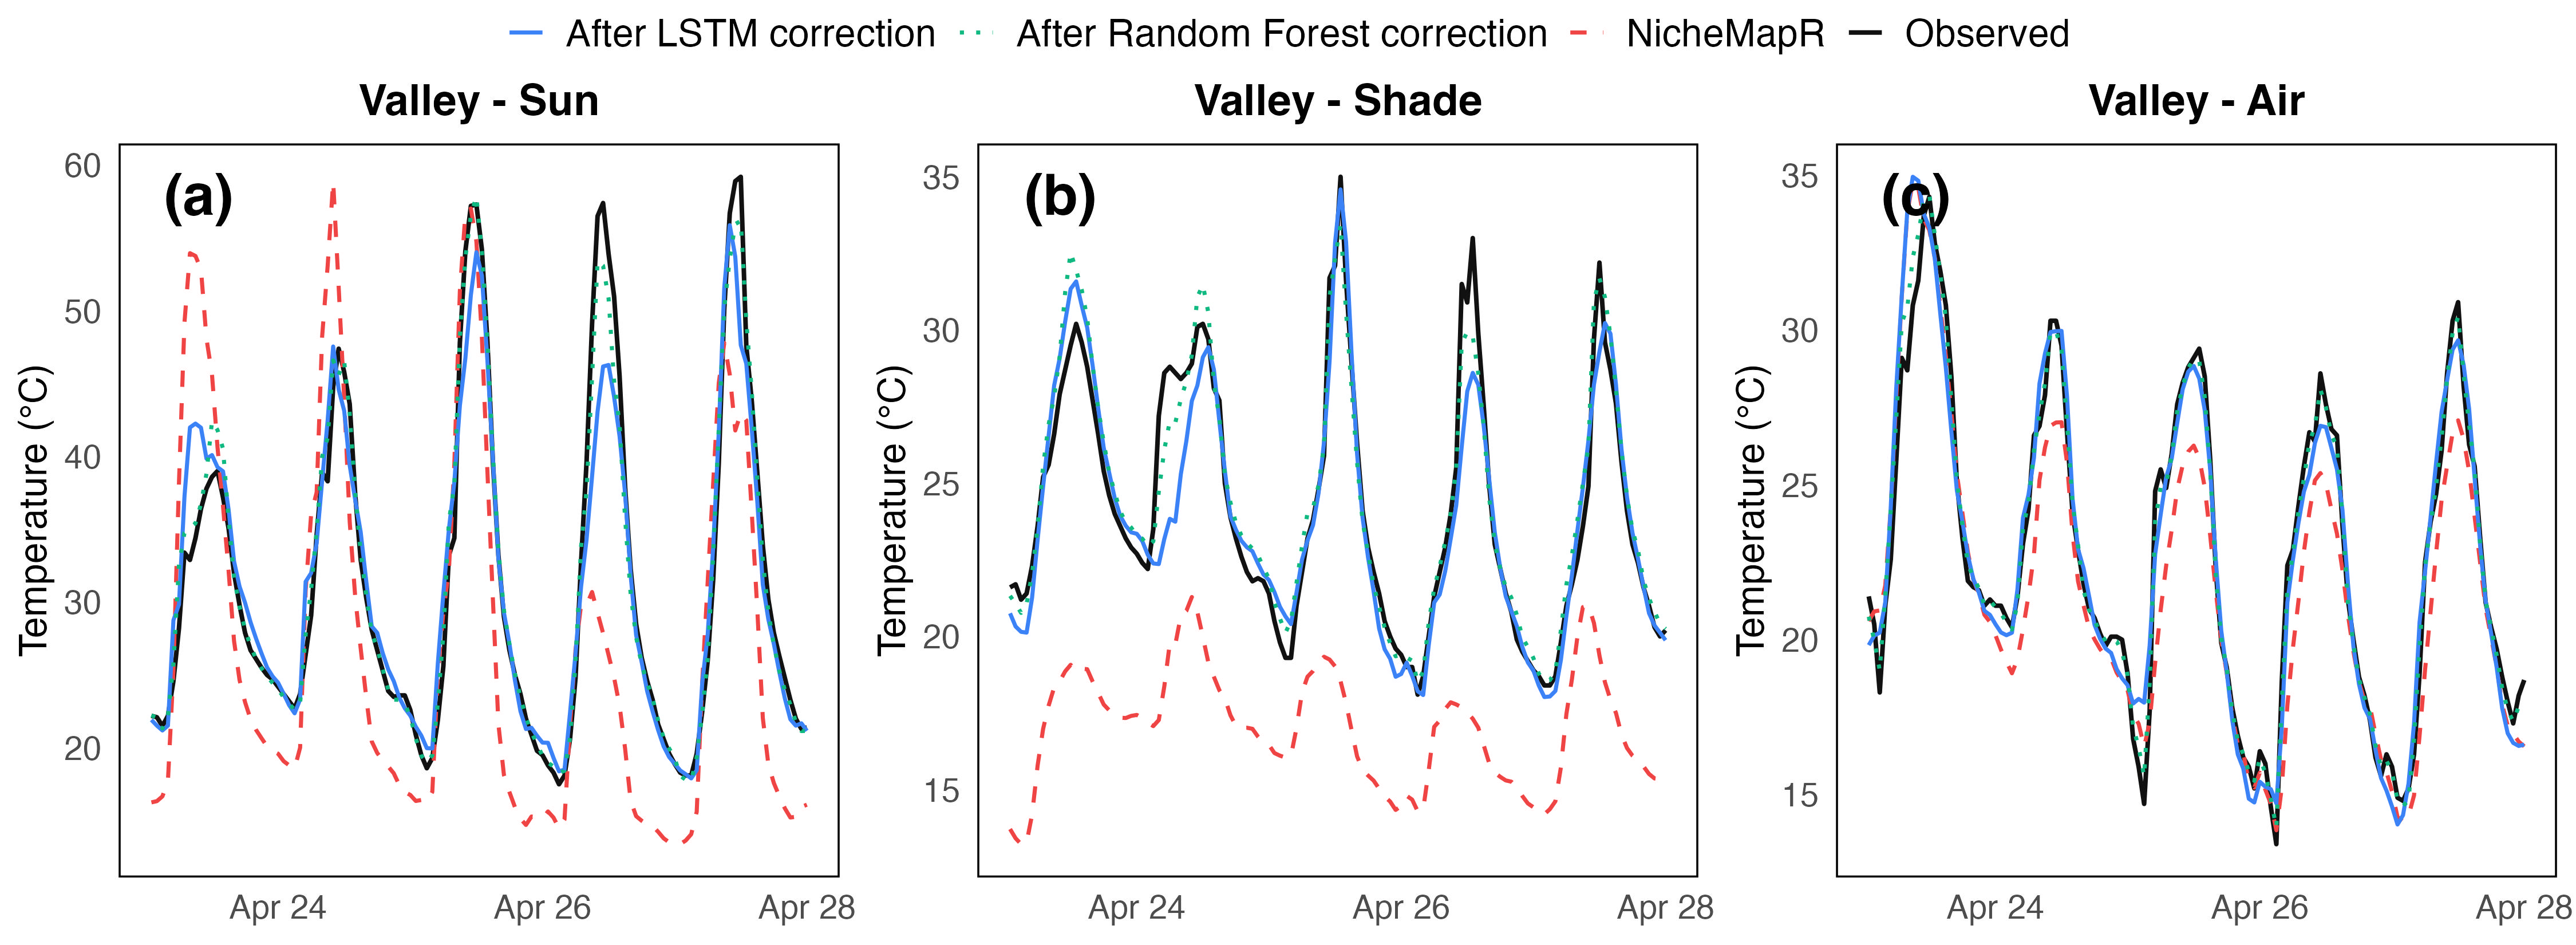
\includegraphics[width=\textwidth,height=0.85\textheight,keepaspectratio]{scenario_1_valley_single_logger/prediction_examples_valley.jpg}
\caption{\textbf{Prediction Examples Valley for Scenario 1.} Time-series prediction examples comparing observed temperatures (black solid line) to the baseline NicheMapR model (red dashed line) and the ML-corrected models (Random Forest in green dotted line, LSTM in blue solid line, if applicable) over a 120-hour window. RF and LSTM perform comparably across microhabitats, with RF having a slight edge on Sun and Shade, while LSTM is marginally better on Air. NicheMapR error is largest for the Sun microhabitat (direct solar exposure), where both models still achieve ~50\% improvement.}
\end{figure}

\clearpage
\begin{figure}[H]
\centering
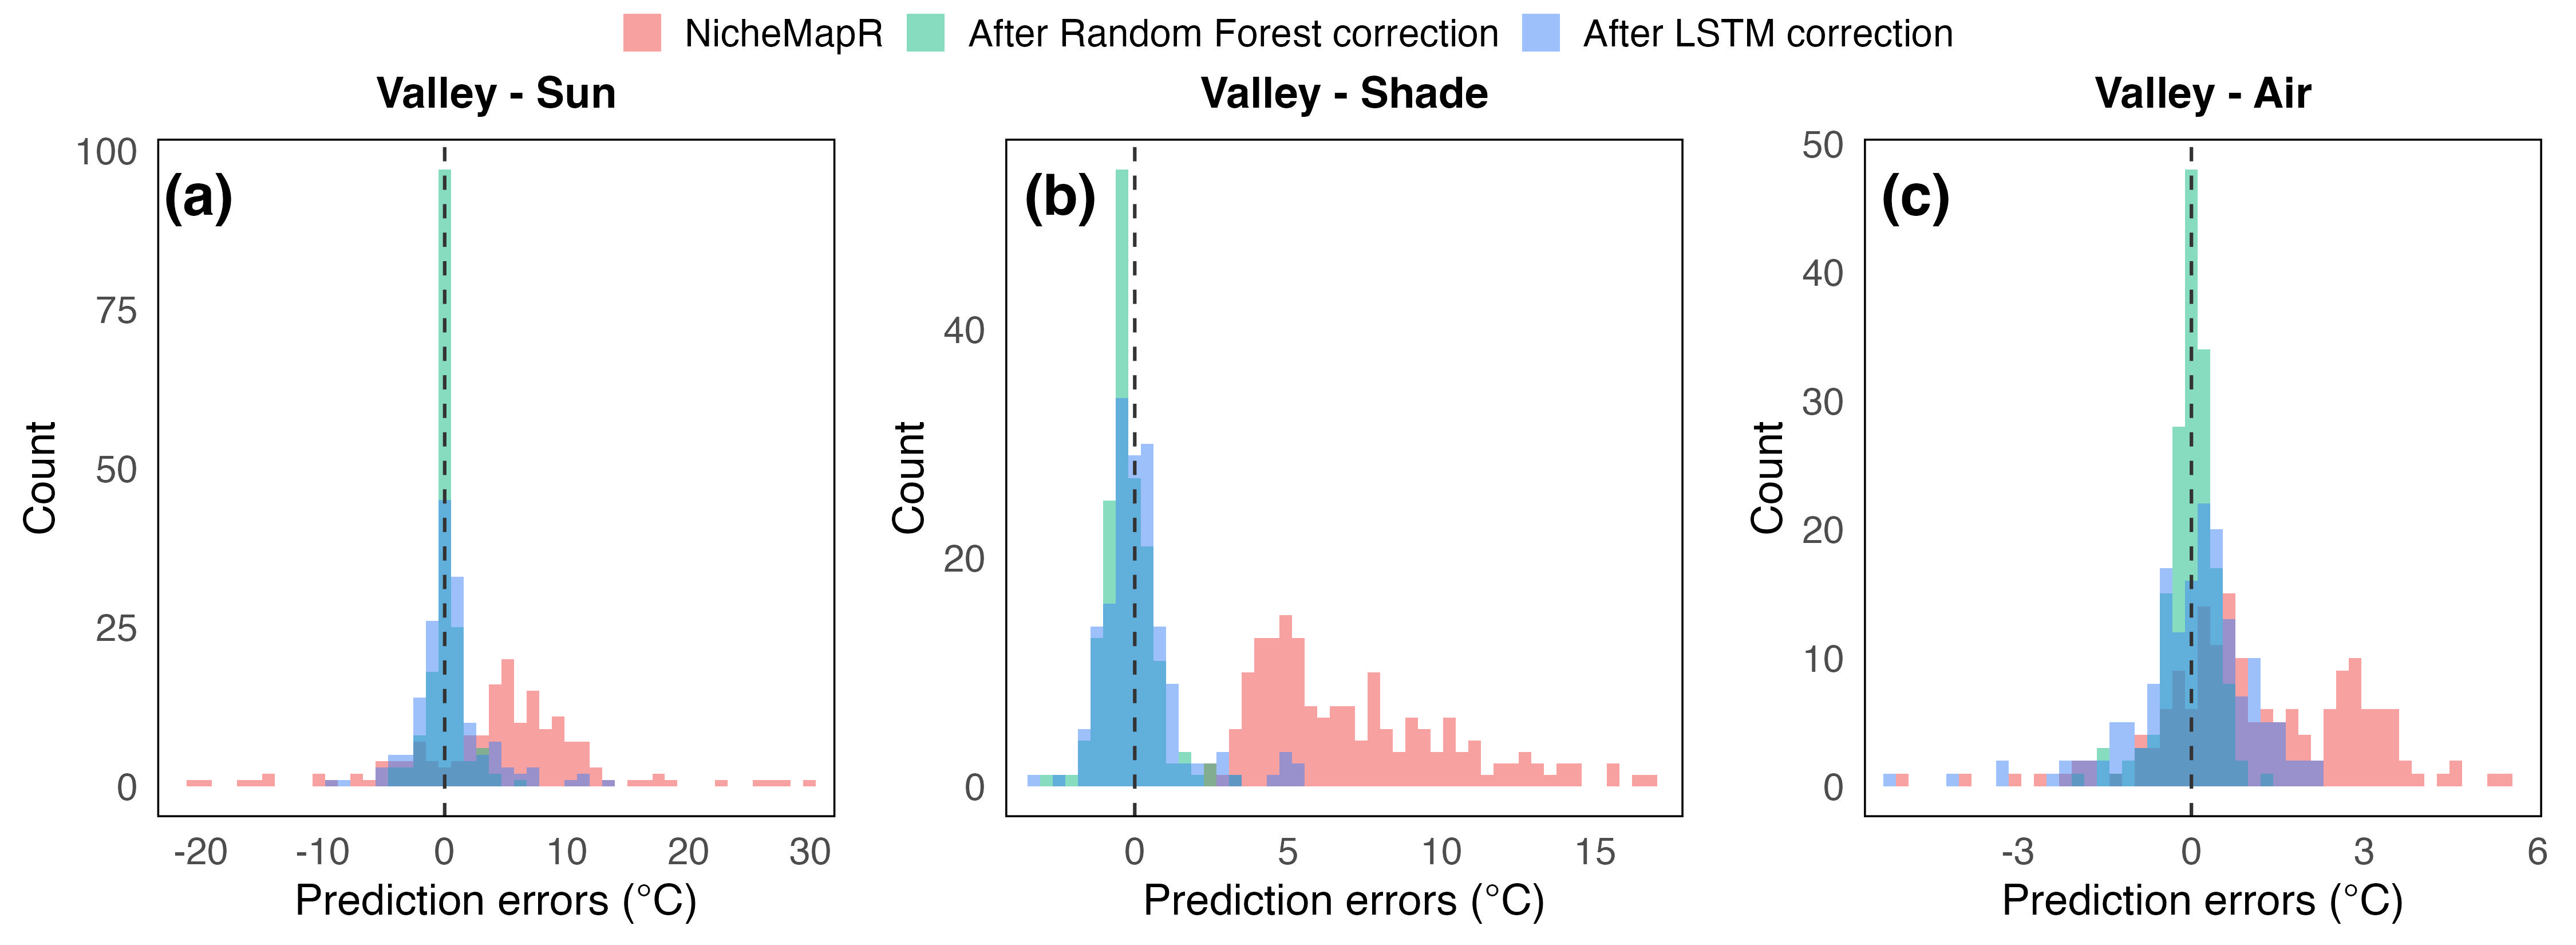
\includegraphics[width=\textwidth,height=0.85\textheight,keepaspectratio]{scenario_1_valley_single_logger/residual_histogram_valley.jpg}
\caption{\textbf{Residual Histogram Valley for Scenario 1.} Distribution of prediction errors (residuals) comparing the baseline NicheMapR model (red) to the ML-corrected models (Random Forest in green, LSTM in blue, if applicable). A narrower distribution centered at zero indicates better performance. RF and LSTM perform comparably across microhabitats, with RF having a slight edge on Sun and Shade, while LSTM is marginally better on Air. NicheMapR error is largest for the Sun microhabitat (direct solar exposure), where both models still achieve ~50\% improvement.}
\end{figure}

\clearpage

\section{Scenario 2: Coastal Beach Habitat (Ashkelon 15 m) Report}

\textbf{Description:} Local correction model trained on a single beach logger (Ashkelon 15 m).
Split: 75\% train / 12.5\% validation / 12.5\% test (random 7-day blocks). Full training set used.

\textbf{Improvement Results:}
\begin{table}[H]
\centering
\begin{tabular}{cccc}
\hline
Model & Baseline NicheMapR RMSE (°C) & Corrected RMSE (°C) & Improvement (\%) \\
\hline
RF & 11.946 & 1.399 & 88.3\% \\
LSTM\_2h & 11.946 & 2.501 & 79.1\% \\
\hline
\end{tabular}
\end{table}


\clearpage
\begin{figure}[H]
\centering
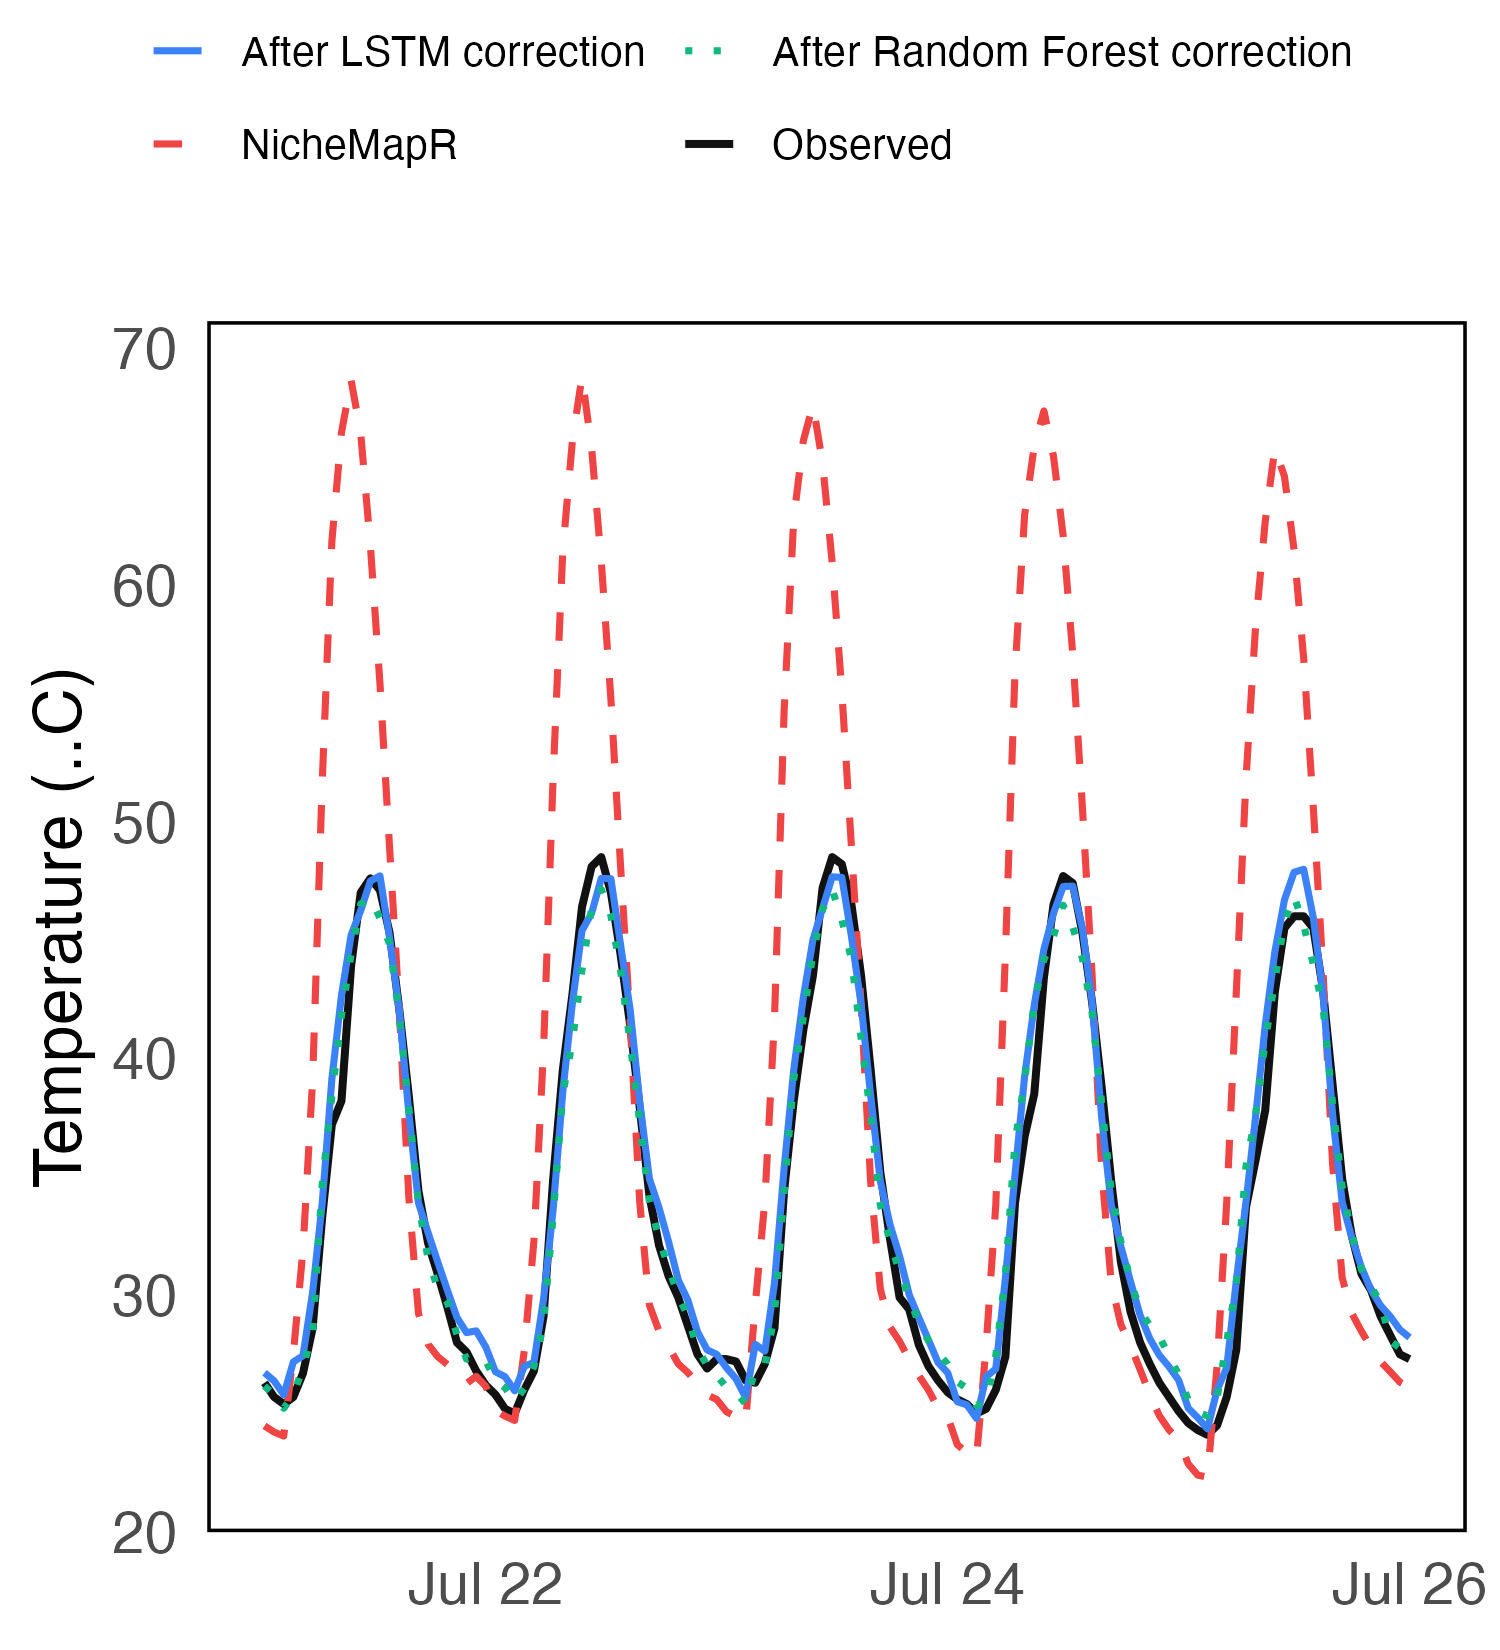
\includegraphics[width=\textwidth,height=0.85\textheight,keepaspectratio]{scenario_2_beach_single_logger/prediction_examples_beach.jpg}
\caption{\textbf{Prediction Examples Beach for Scenario 2.} Time-series prediction examples comparing observed temperatures (black solid line) to the baseline NicheMapR model (red dashed line) and the ML-corrected models (Random Forest in green dotted line, LSTM in blue solid line, if applicable) over a 120-hour window. RF outperforms LSTM at this training set size. Both achieve large improvements over the NicheMapR baseline (~79–88\%), demonstrating that even a single beach logger provides sufficient signal to substantially reduce coastal microclimate errors.}
\end{figure}

\clearpage
\begin{figure}[H]
\centering
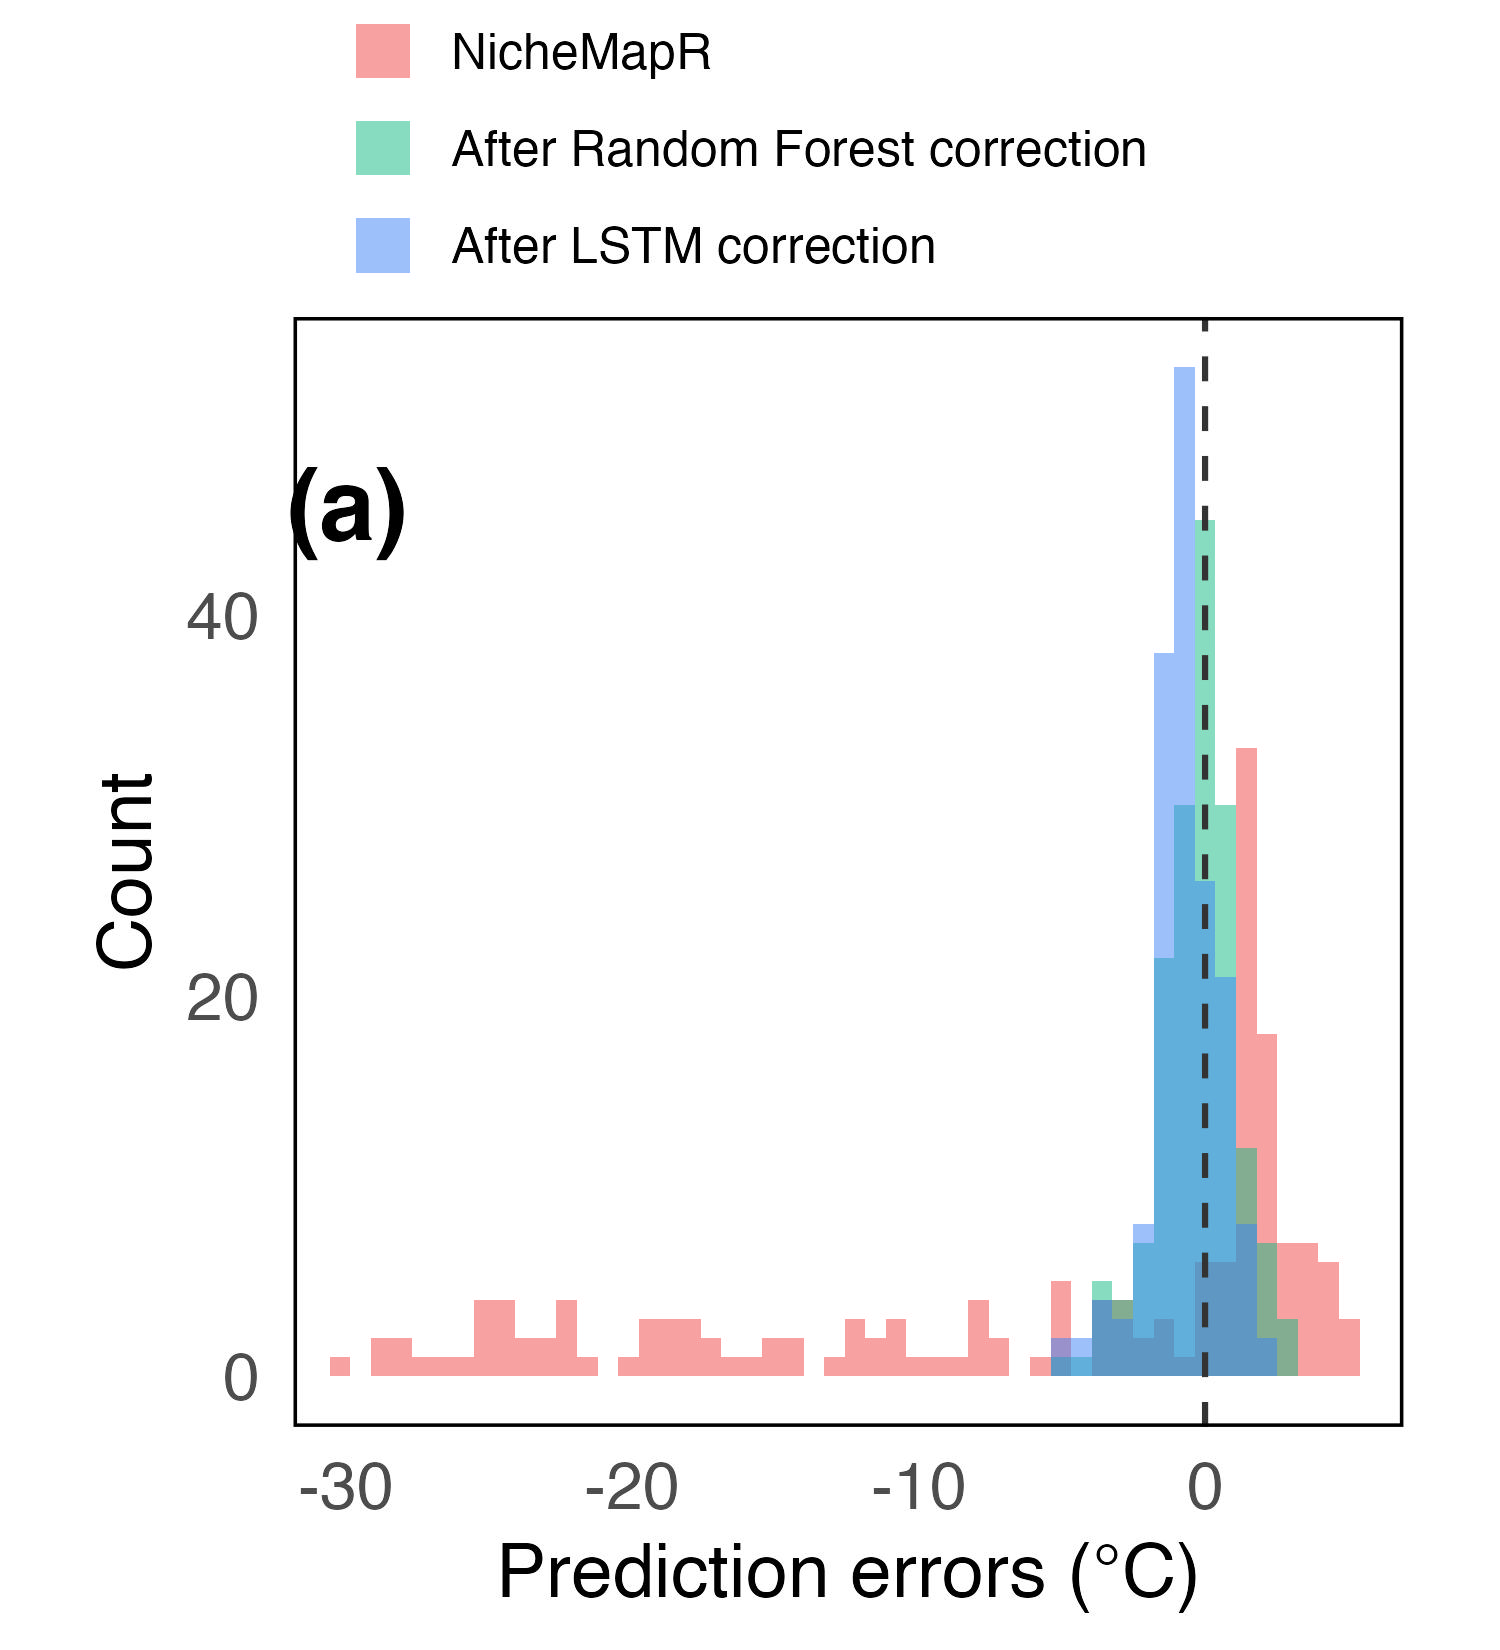
\includegraphics[width=\textwidth,height=0.85\textheight,keepaspectratio]{scenario_2_beach_single_logger/residual_histogram_beach.jpg}
\caption{\textbf{Residual Histogram Beach for Scenario 2.} Distribution of prediction errors (residuals) comparing the baseline NicheMapR model (red) to the ML-corrected models (Random Forest in green, LSTM in blue, if applicable). A narrower distribution centered at zero indicates better performance. RF outperforms LSTM at this training set size. Both achieve large improvements over the NicheMapR baseline (~79–88\%), demonstrating that even a single beach logger provides sufficient signal to substantially reduce coastal microclimate errors.}
\end{figure}

\clearpage

\section{Scenario 3: Judean Desert Habitat (Tzeelim) Report}

\textbf{Description:} Local correction models trained on two microhabitats (Rock, Bush) at the Tzeelim desert site.
Split: 75\% train / 12.5\% validation / 12.5\% test (random 7-day blocks). Full training set used.

\textbf{Improvement Results:}
\begin{table}[H]
\centering
\begin{tabular}{cccccc}
\hline
Microhabitat & Baseline NicheMapR RMSE (°C) & RF RMSE (°C) & RF Imp (\%) & LSTM (2h) RMSE (°C) & LSTM (2h) Imp (\%) \\
\hline
Rock & 6.536 & 1.657 & 74.6\% & 2.156 & 67.0\% \\
Bush & 6.344 & 2.090 & 67.1\% & 1.619 & 74.5\% \\
\textbf{Average} & \textbf{6.440} & \textbf{1.873} & \textbf{70.9\%} & \textbf{1.888} & \textbf{70.7\%} \\
\hline
\end{tabular}
\end{table}


\clearpage
\begin{figure}[H]
\centering
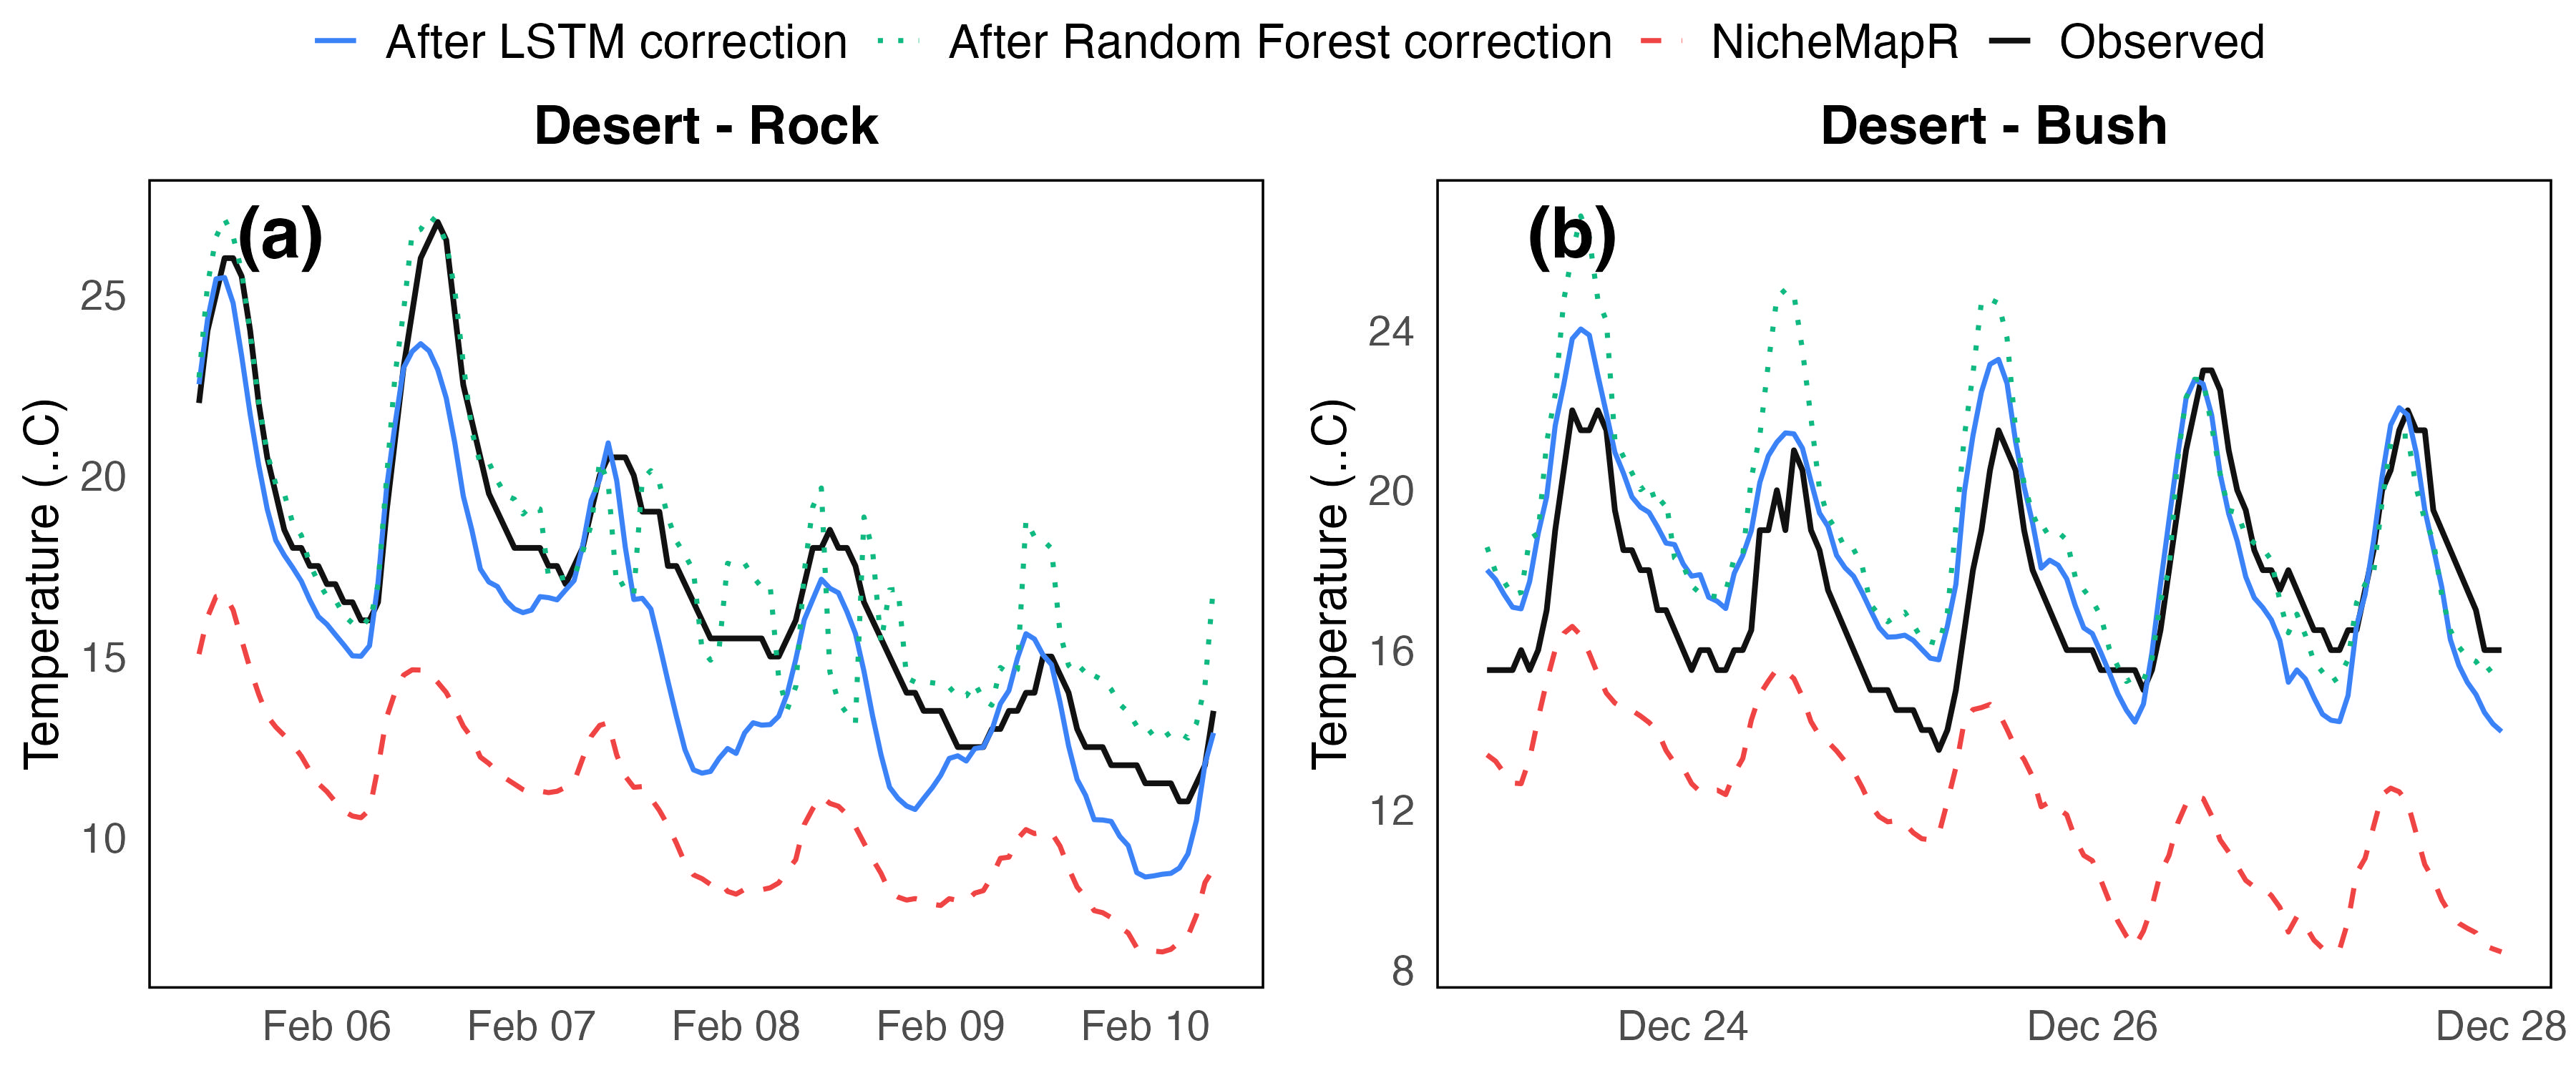
\includegraphics[width=\textwidth,height=0.85\textheight,keepaspectratio]{scenario_3_desert_single_logger/prediction_examples_desert.jpg}
\caption{\textbf{Prediction Examples Desert for Scenario 3.} Time-series prediction examples comparing observed temperatures (black solid line) to the baseline NicheMapR model (red dashed line) and the ML-corrected models (Random Forest in green dotted line, LSTM in blue solid line, if applicable) over a 120-hour window. RF and LSTM perform comparably on average (~71\% improvement each), with RF leading on Rock and LSTM leading on Bush. The NicheMapR baseline error is large (~6.4 °C) due to complex rock and bush surface energy balance; both models correct it substantially.}
\end{figure}

\clearpage
\begin{figure}[H]
\centering
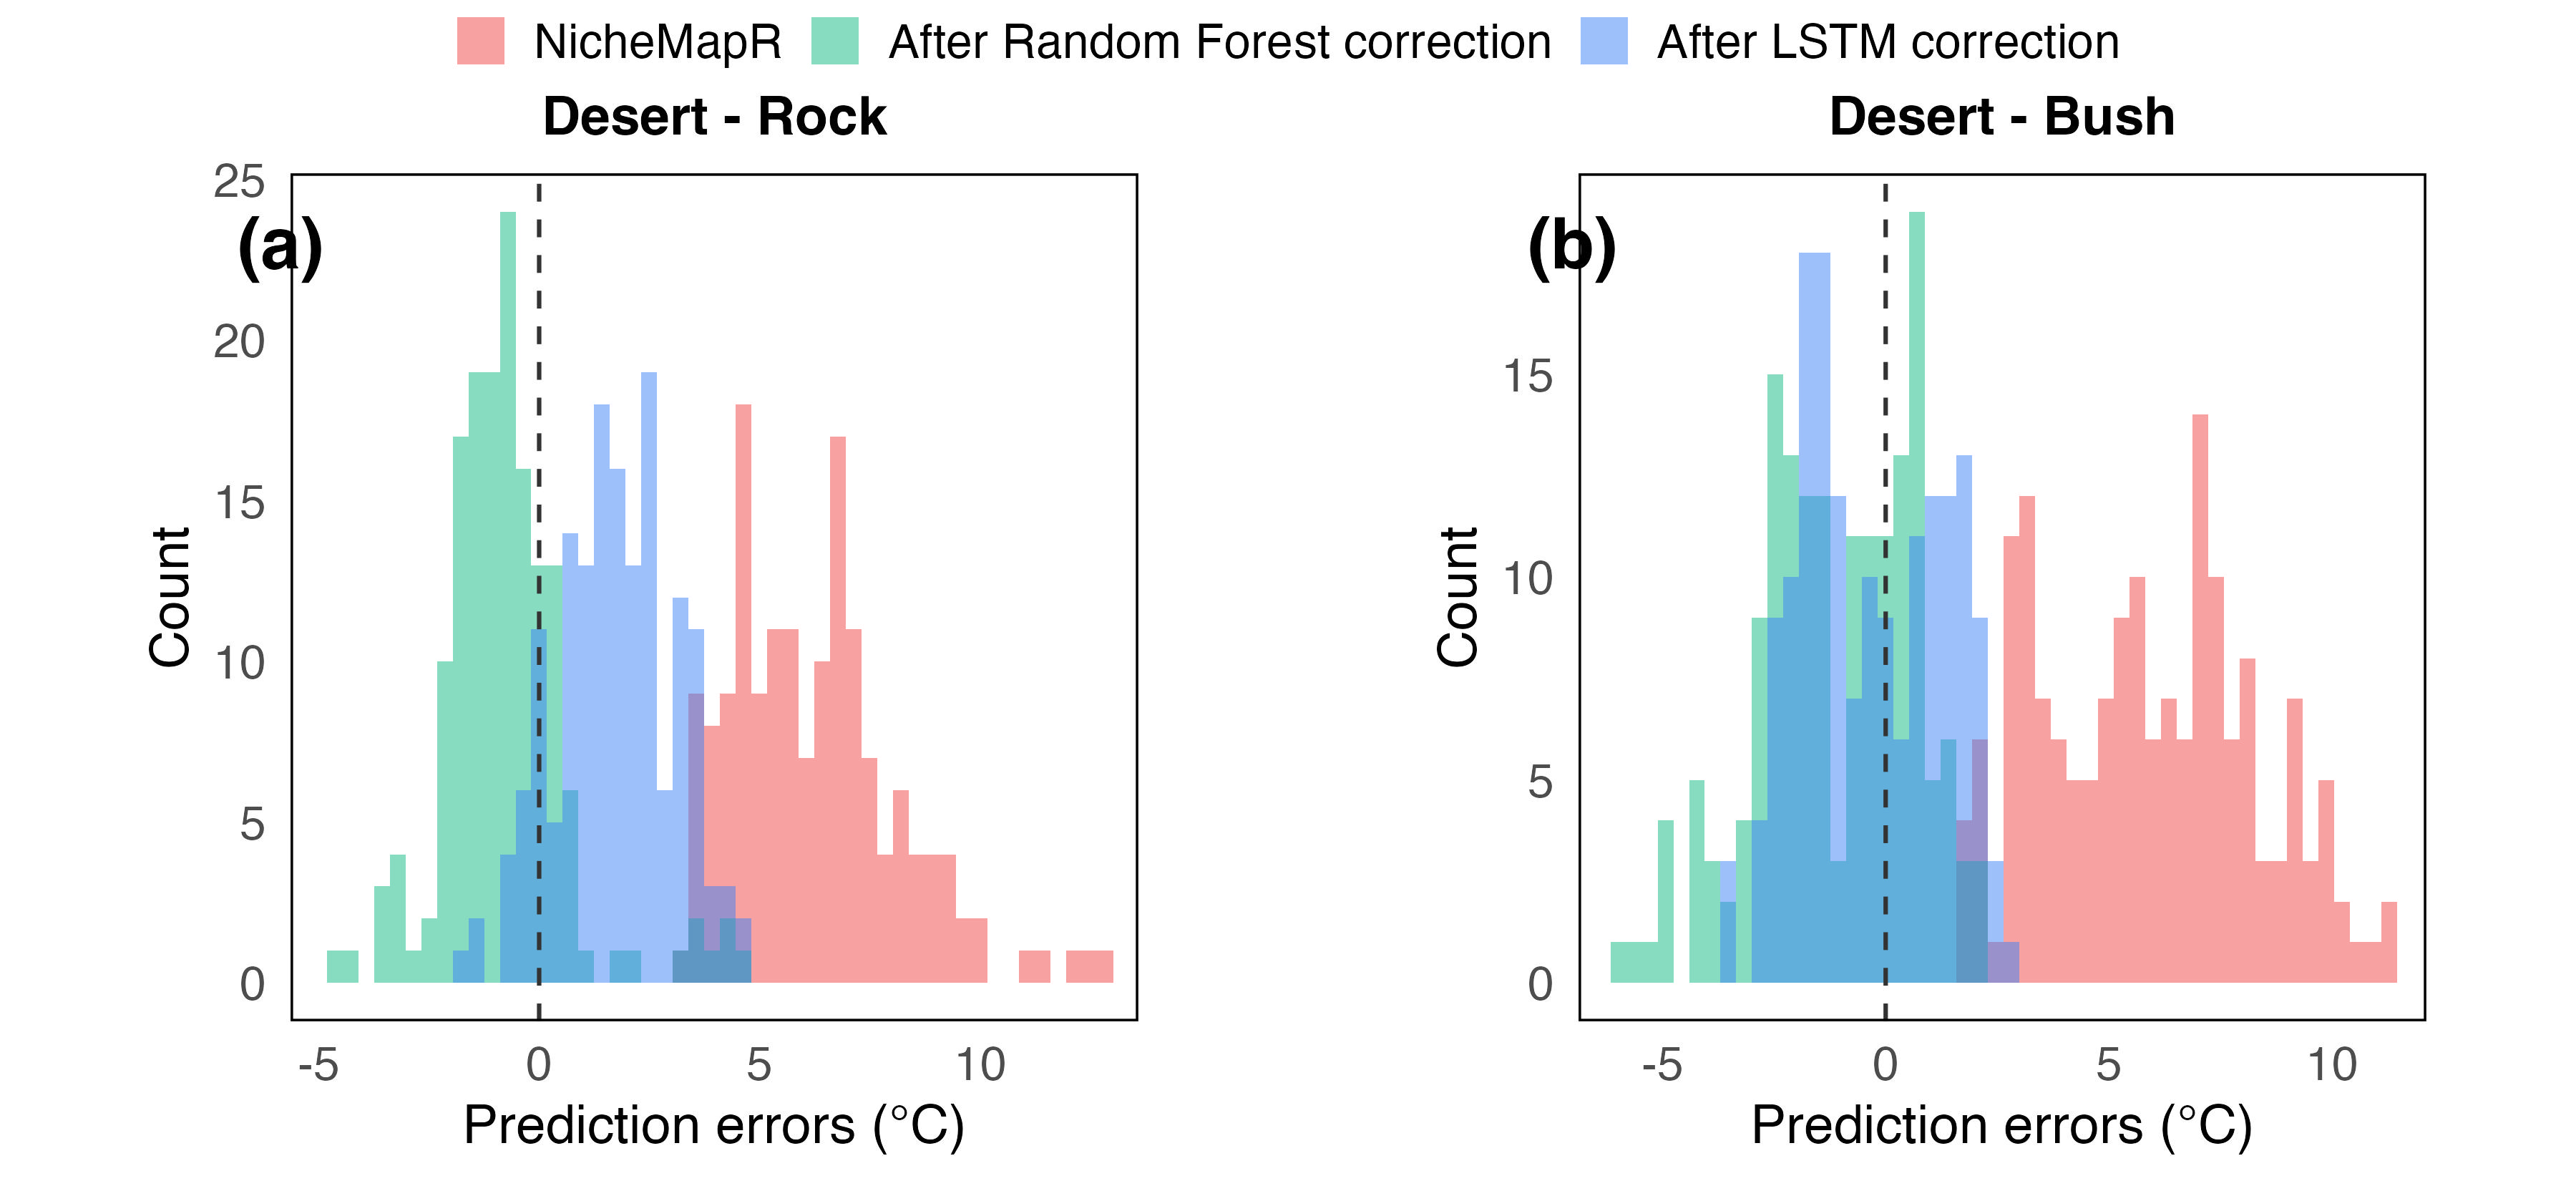
\includegraphics[width=\textwidth,height=0.85\textheight,keepaspectratio]{scenario_3_desert_single_logger/residual_histogram_desert.jpg}
\caption{\textbf{Residual Histogram Desert for Scenario 3.} Distribution of prediction errors (residuals) comparing the baseline NicheMapR model (red) to the ML-corrected models (Random Forest in green, LSTM in blue, if applicable). A narrower distribution centered at zero indicates better performance. RF and LSTM perform comparably on average (~71\% improvement each), with RF leading on Rock and LSTM leading on Bush. The NicheMapR baseline error is large (~6.4 °C) due to complex rock and bush surface energy balance; both models correct it substantially.}
\end{figure}

\clearpage

\section{Scenario 4: Beach Habitat — Pooled Spatial Generalization}

\textbf{Description:} A single unified model is trained on all 7 beach logger sites combined and evaluated on each individual site.

**Comparison baseline — Scenario 2 (single logger):** RF RMSE = 3.06 °C, improvement = 62.6\%,
trained on ~1,405 rows (Ashkelon 15 m only).
The pooled model uses ~10× more training data, so performance gains cannot be attributed
solely to spatial diversity (see Scenario 8 for a controlled comparison).

\textbf{Sample Sizes:}
\begin{table}[H]
\centering
\begin{tabular}{cc}
\hline
Split & Rows \\
\hline
Train & 13,988 \\
Validation & 4,210 \\
Test & 4,487 \\
\hline
\end{tabular}
\end{table}


\clearpage
\begin{figure}[H]
\centering
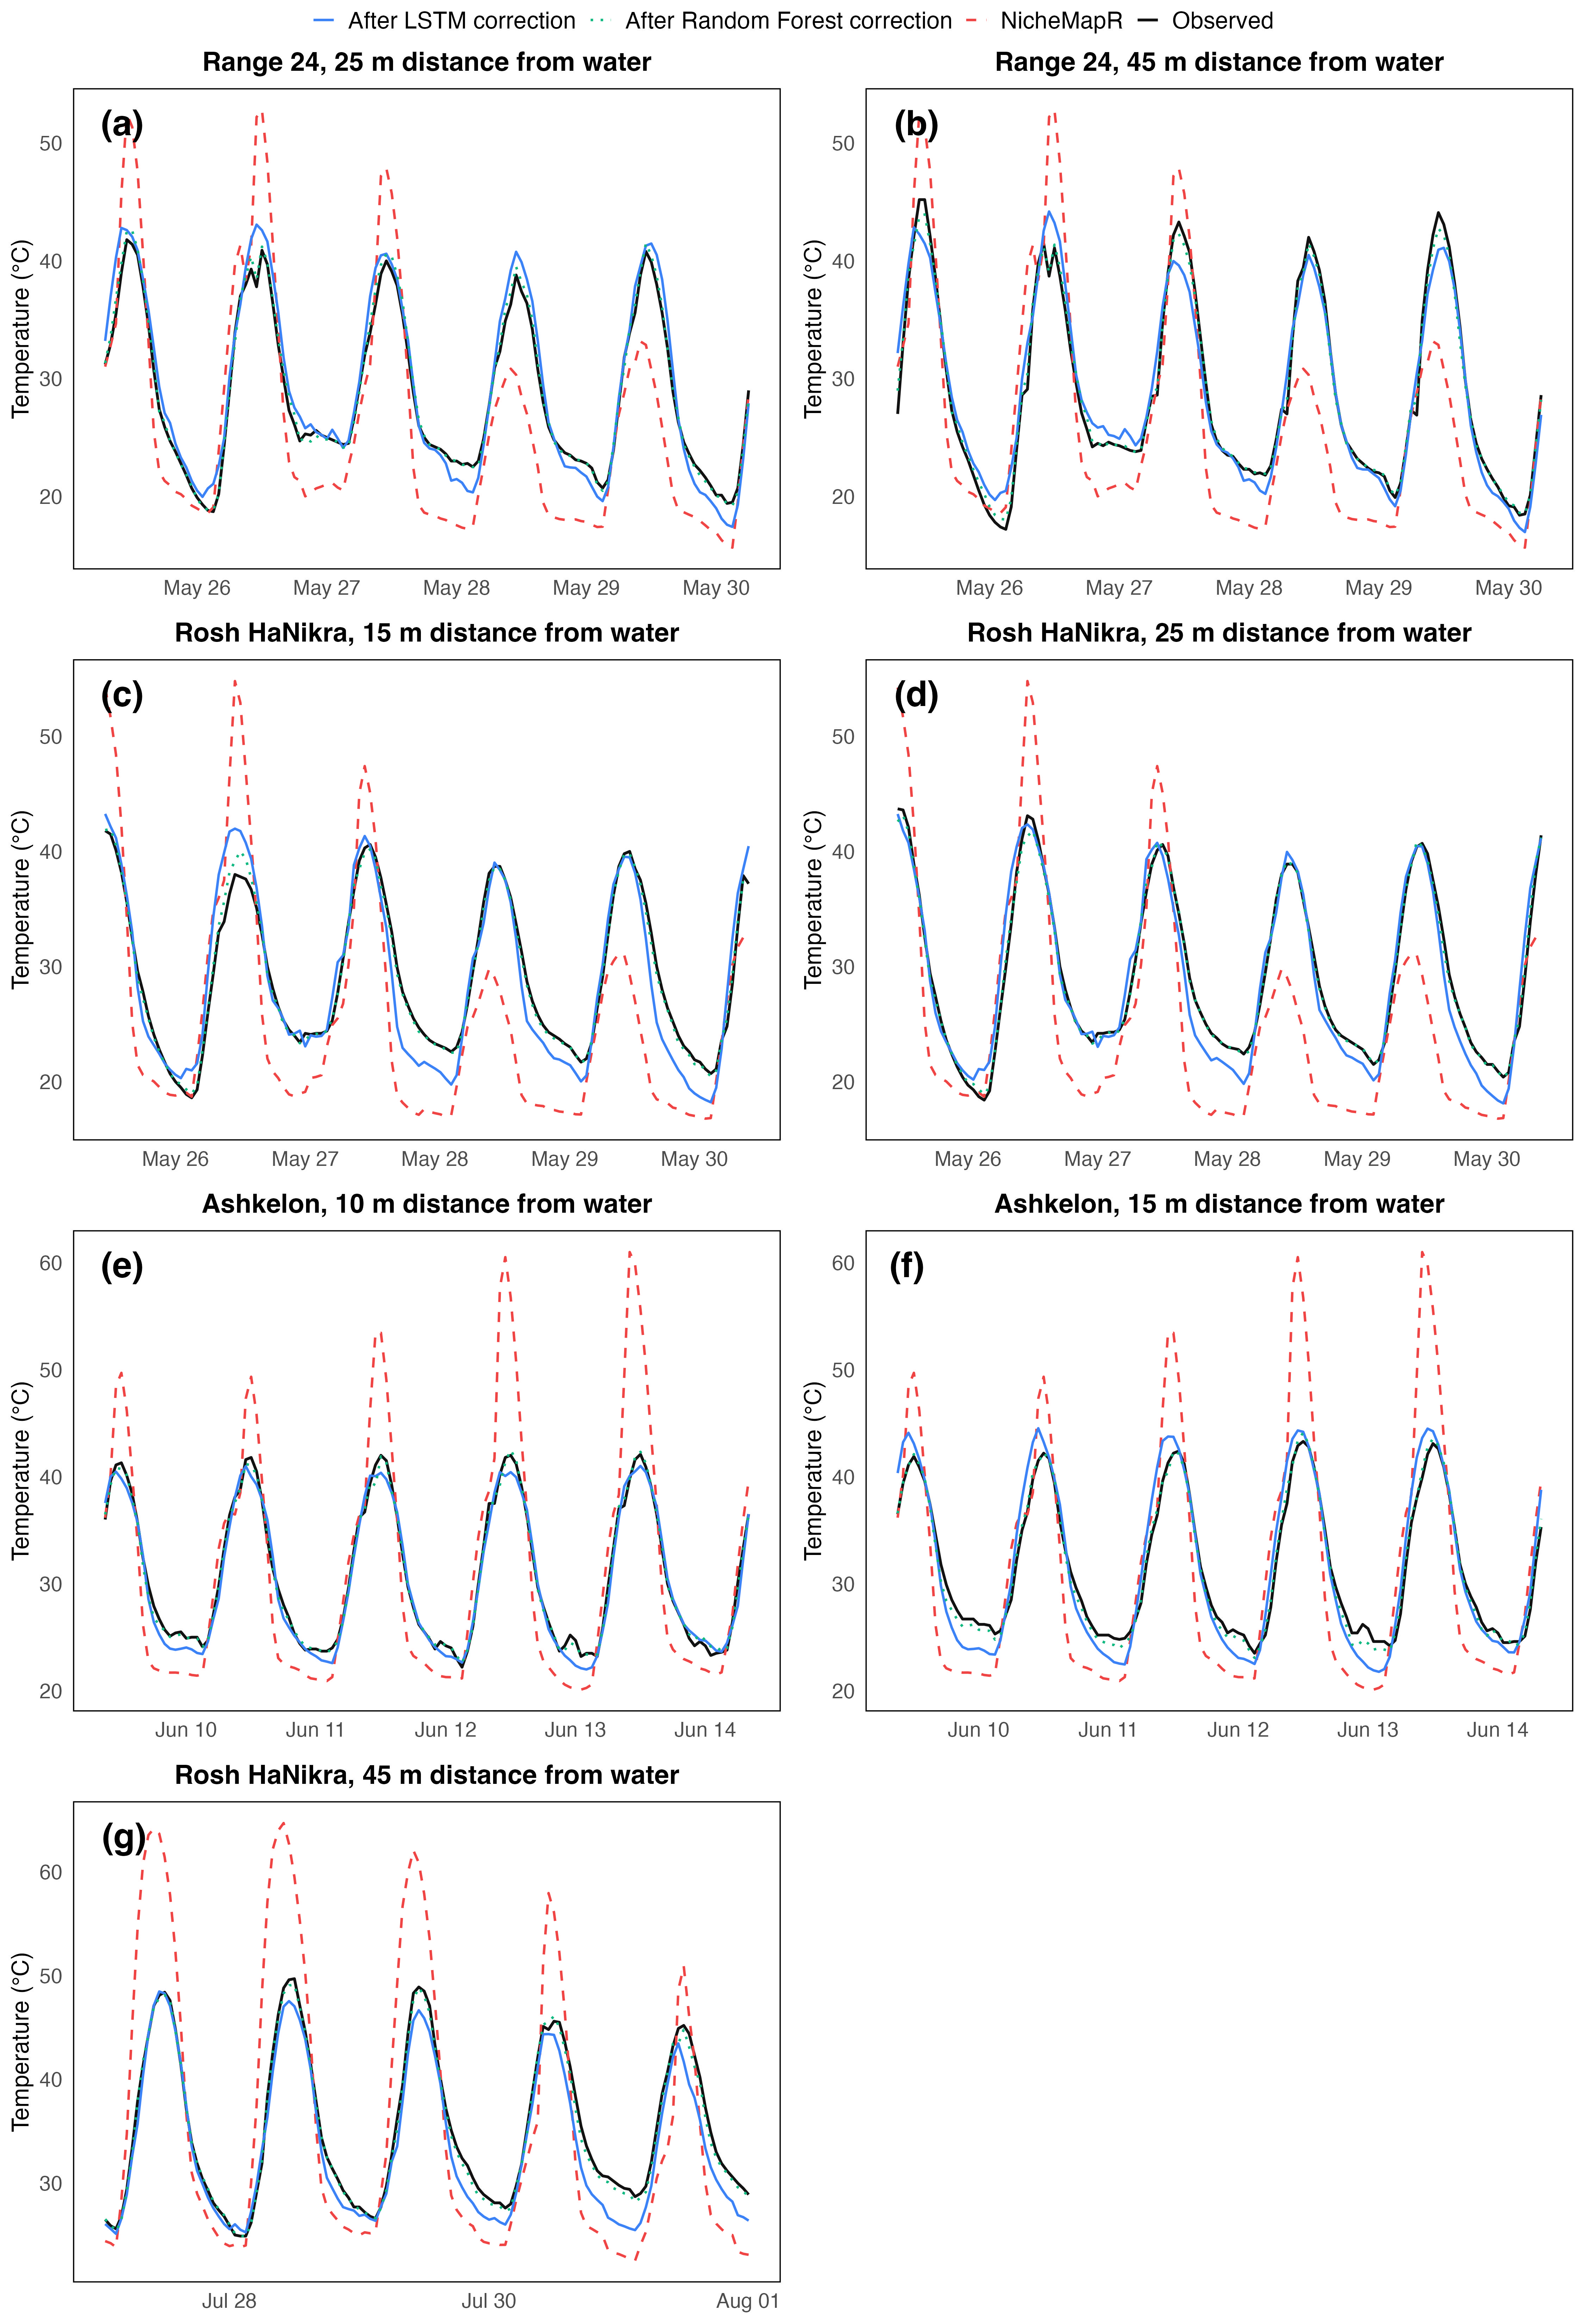
\includegraphics[width=\textwidth,height=0.85\textheight,keepaspectratio]{scenario_4_beach_pooled/prediction_examples_beach_pooled.jpg}
\caption{\textbf{Prediction Examples Beach Pooled for Scenario 4.} Time-series prediction examples comparing observed temperatures (black solid line) to the baseline NicheMapR model (red dashed line) and the ML-corrected models (Random Forest in green dotted line, LSTM in blue solid line, if applicable) over a 120-hour window. The pooled RF model (avg 0.875 °C, 89.7\% improvement) substantially outperforms the single-logger baseline from Scenario 2 (3.06 °C, 62.6\%), but has ~10× more training data, so the comparison is not volume-controlled. Performance is virtually identical to the specialized per-location models in Scenario 5 (~0.84 °C avg), confirming that a single pooled model generalizes as well as separate location-specific models.}
\end{figure}

\clearpage
\begin{figure}[H]
\centering
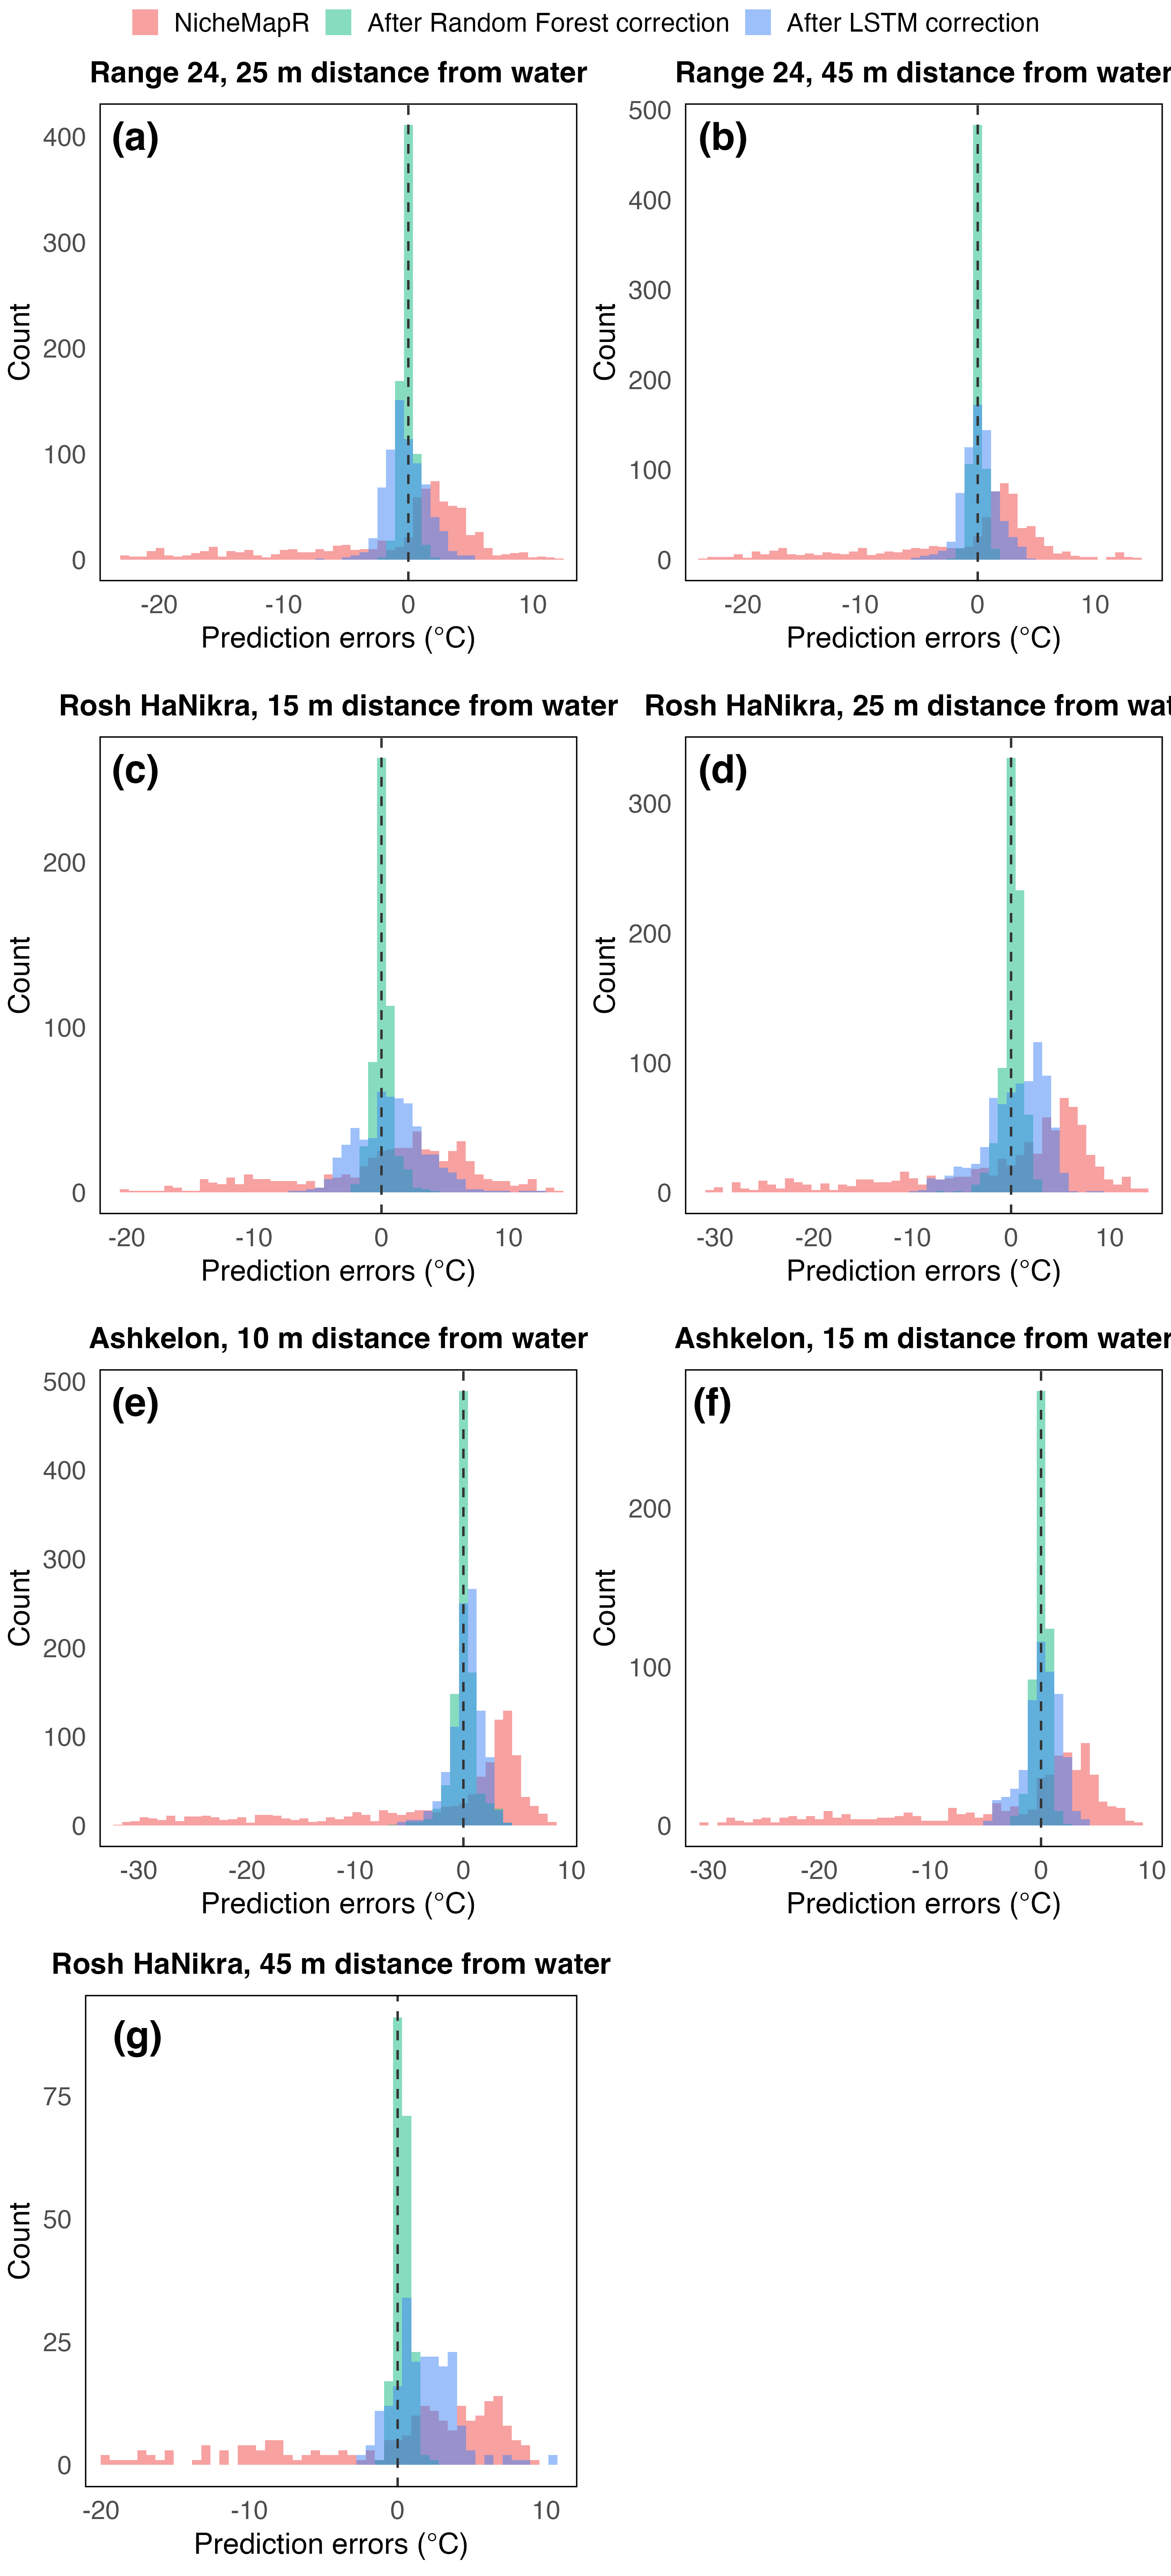
\includegraphics[width=\textwidth,height=0.85\textheight,keepaspectratio]{scenario_4_beach_pooled/residual_histogram_beach_pooled.jpg}
\caption{\textbf{Residual Histogram Beach Pooled for Scenario 4.} Distribution of prediction errors (residuals) comparing the baseline NicheMapR model (red) to the ML-corrected models (Random Forest in green, LSTM in blue, if applicable). A narrower distribution centered at zero indicates better performance. The pooled RF model (avg 0.875 °C, 89.7\% improvement) substantially outperforms the single-logger baseline from Scenario 2 (3.06 °C, 62.6\%), but has ~10× more training data, so the comparison is not volume-controlled. Performance is virtually identical to the specialized per-location models in Scenario 5 (~0.84 °C avg), confirming that a single pooled model generalizes as well as separate location-specific models.}
\end{figure}

\clearpage

\section{Scenario 5: Beach Habitat — Specialized (Location-Specific) Models}

\textbf{Description:} Location-specific models are trained on each of the three coastal locations (Ashkelon, Range 24, Rosh HaNikra) and tested on local sensor sites.

**Comparison baselines:**
- Scenario 2 (single logger, Ashkelon 15 m only): RF RMSE = 3.06 °C, 62.6\% improvement, ~1,405 train rows.
- Scenario 4 (pooled, all 7 loggers): RF avg RMSE = 0.875 °C, 89.7\% improvement, 13,988 train rows.

\clearpage
\begin{figure}[H]
\centering
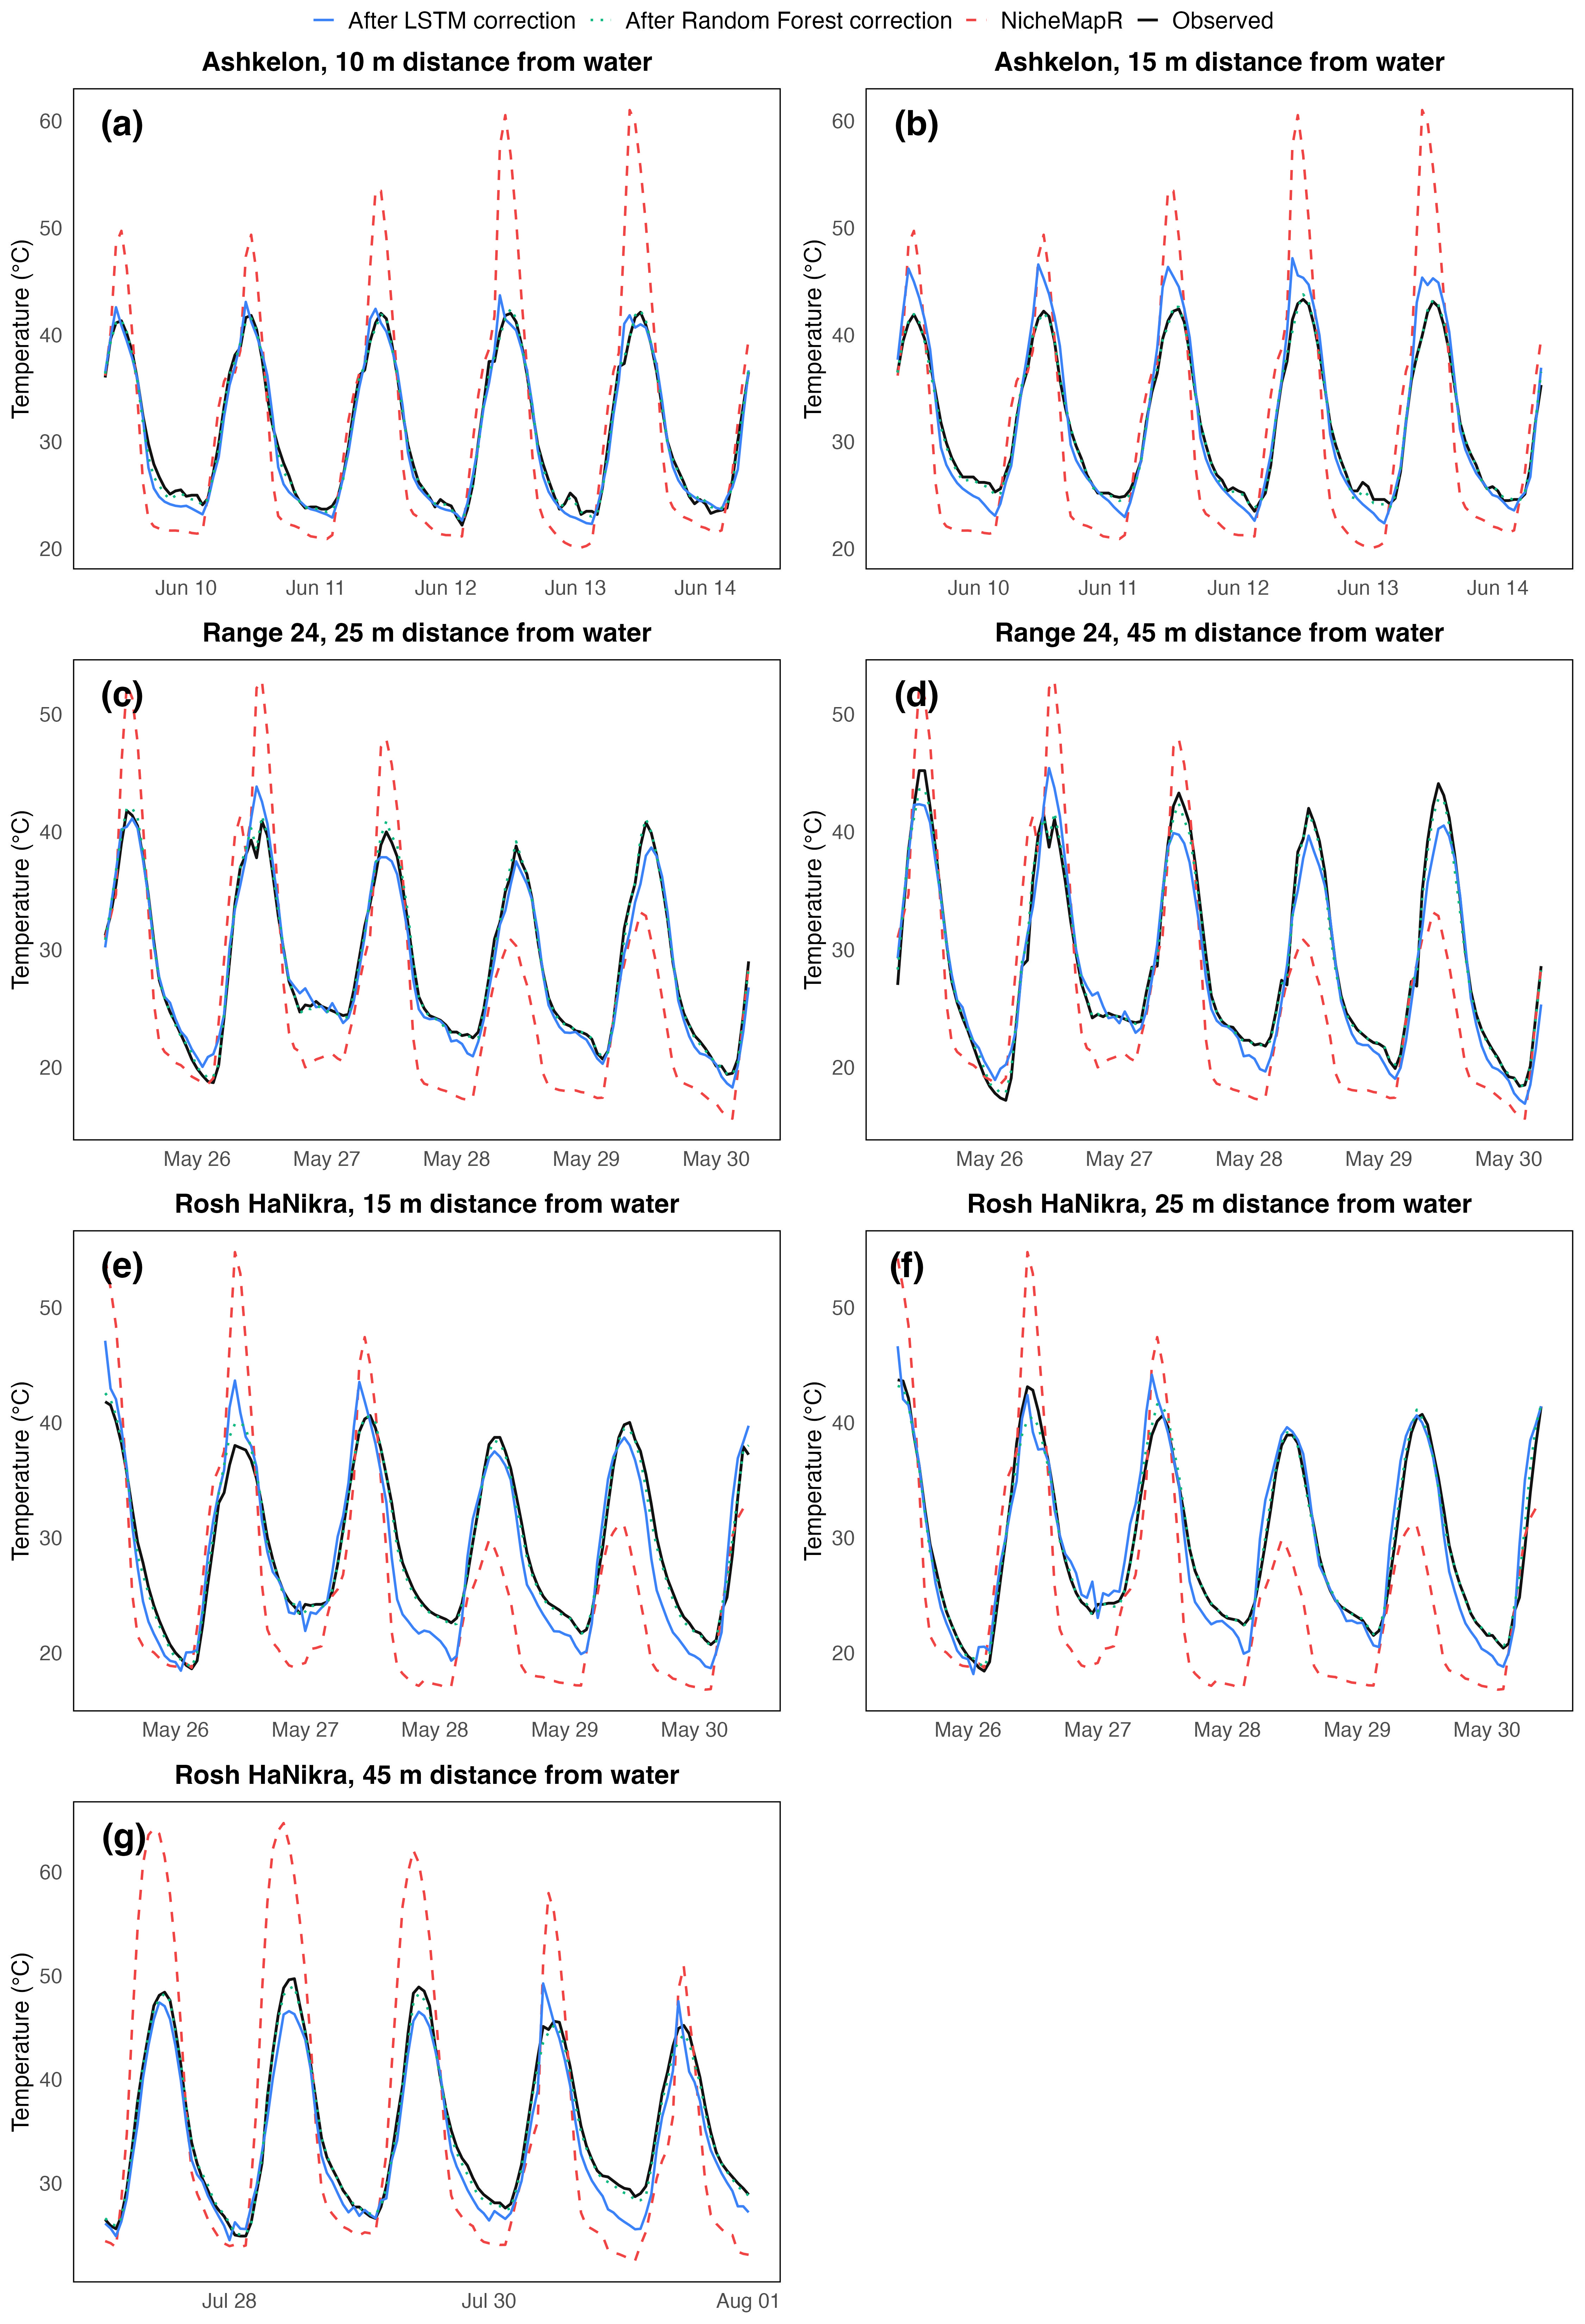
\includegraphics[width=\textwidth,height=0.85\textheight,keepaspectratio]{scenario_5_beach_specialized/prediction_examples_beach_specialized.jpg}
\caption{\textbf{Prediction Examples Beach Specialized for Scenario 5.} Time-series prediction examples comparing observed temperatures (black solid line) to the baseline NicheMapR model (red dashed line) and the ML-corrected models (Random Forest in green dotted line, LSTM in blue solid line, if applicable) over a 120-hour window. Specialized RF models (avg ~0.84 °C, ~90\% improvement) substantially outperform the single-logger baseline from Scenario 2 (3.06 °C, 62.6\%), but use ~3× more training data per location (4,464–4,893 rows vs ~1,405 rows), making it a volume-confounded comparison. Performance is virtually identical to the pooled model in Scenario 4 (0.875 °C), which uses all 13,988 rows — confirming that location-specific pooling captures most of the benefit of the full pooled model while using only a third of the data.}
\end{figure}

\clearpage
\begin{figure}[H]
\centering
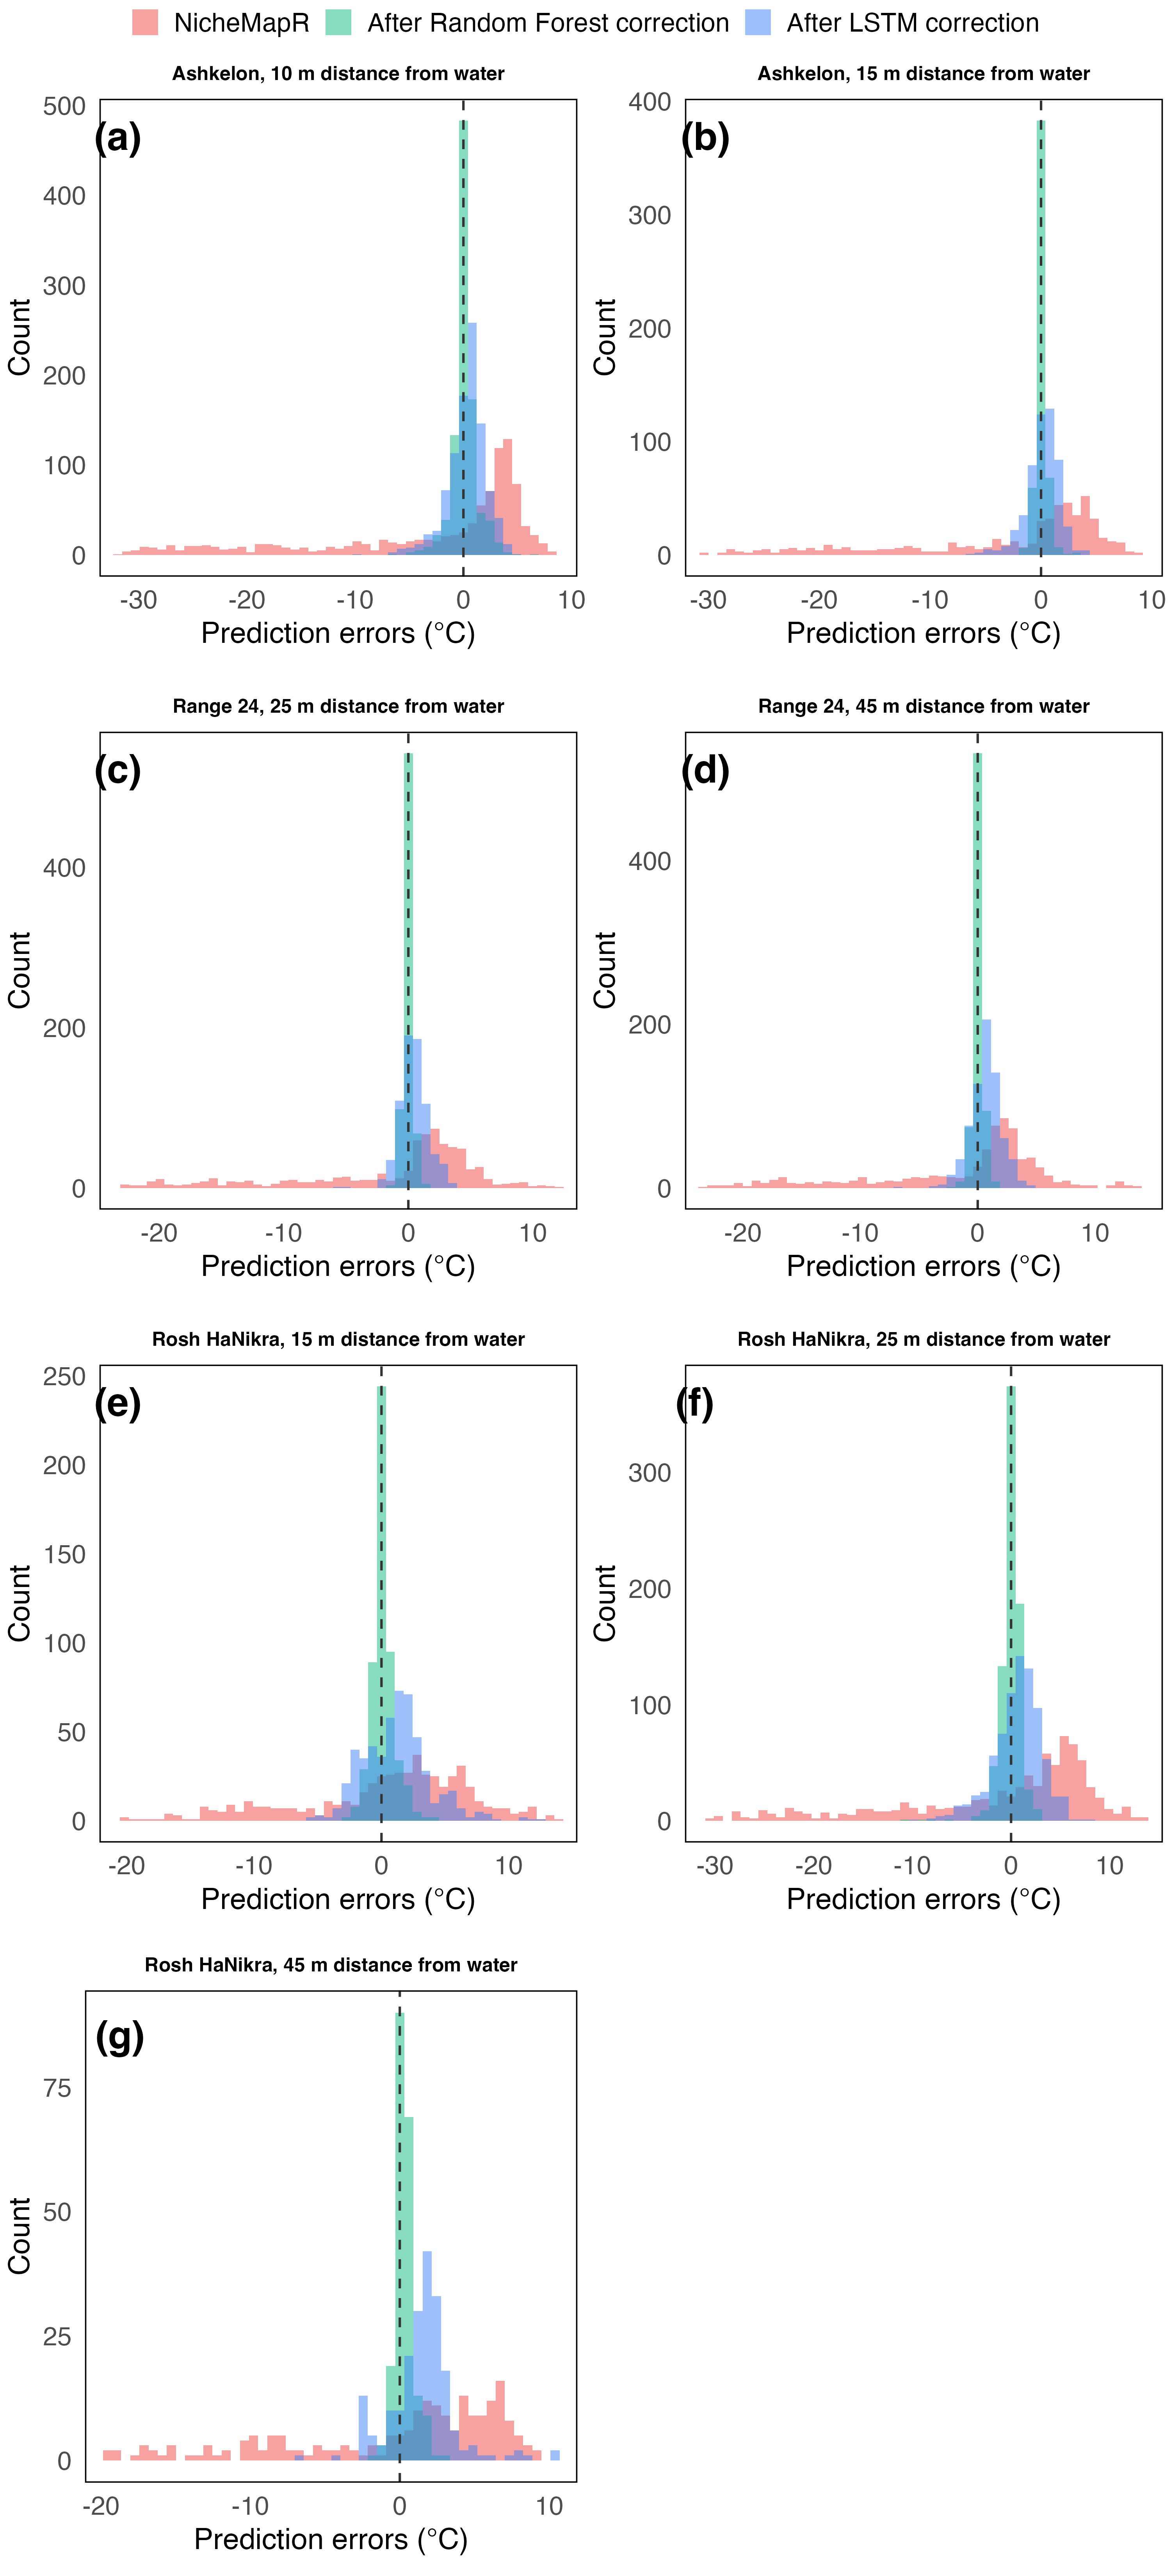
\includegraphics[width=\textwidth,height=0.85\textheight,keepaspectratio]{scenario_5_beach_specialized/residual_histogram_beach_specialized.jpg}
\caption{\textbf{Residual Histogram Beach Specialized for Scenario 5.} Distribution of prediction errors (residuals) comparing the baseline NicheMapR model (red) to the ML-corrected models (Random Forest in green, LSTM in blue, if applicable). A narrower distribution centered at zero indicates better performance. Specialized RF models (avg ~0.84 °C, ~90\% improvement) substantially outperform the single-logger baseline from Scenario 2 (3.06 °C, 62.6\%), but use ~3× more training data per location (4,464–4,893 rows vs ~1,405 rows), making it a volume-confounded comparison. Performance is virtually identical to the pooled model in Scenario 4 (0.875 °C), which uses all 13,988 rows — confirming that location-specific pooling captures most of the benefit of the full pooled model while using only a third of the data.}
\end{figure}

\clearpage

\section{Scenario 6: Judean Desert — Pooled Spatial Generalization}

\textbf{Description:} A single unified model trained on all 48 Judean Desert loggers is evaluated per site and aggregated by Region (Mishmar vs Tzeelim) and Microhabitat (Bush vs Rock).

**Comparison baseline — Scenario 3 (single loggers):** RF RMSE = 1.884 °C overall, 73.9\% improvement,
trained on ~448 rows (Rock\_S\_T\_2\_W) and ~1,570 rows (Bush\_S\_T\_2\_W) respectively.
The pooled model uses 118,753 training rows — far more data — so the performance gain
is volume-confounded and cannot be attributed to spatial diversity alone.

\textbf{Sample Sizes:}
\begin{table}[H]
\centering
\begin{tabular}{cc}
\hline
Split & Rows \\
\hline
Train & 118,753 \\
Validation & 23,148 \\
Test & 33,486 \\
\hline
\end{tabular}
\end{table}


\clearpage
\begin{figure}[H]
\centering
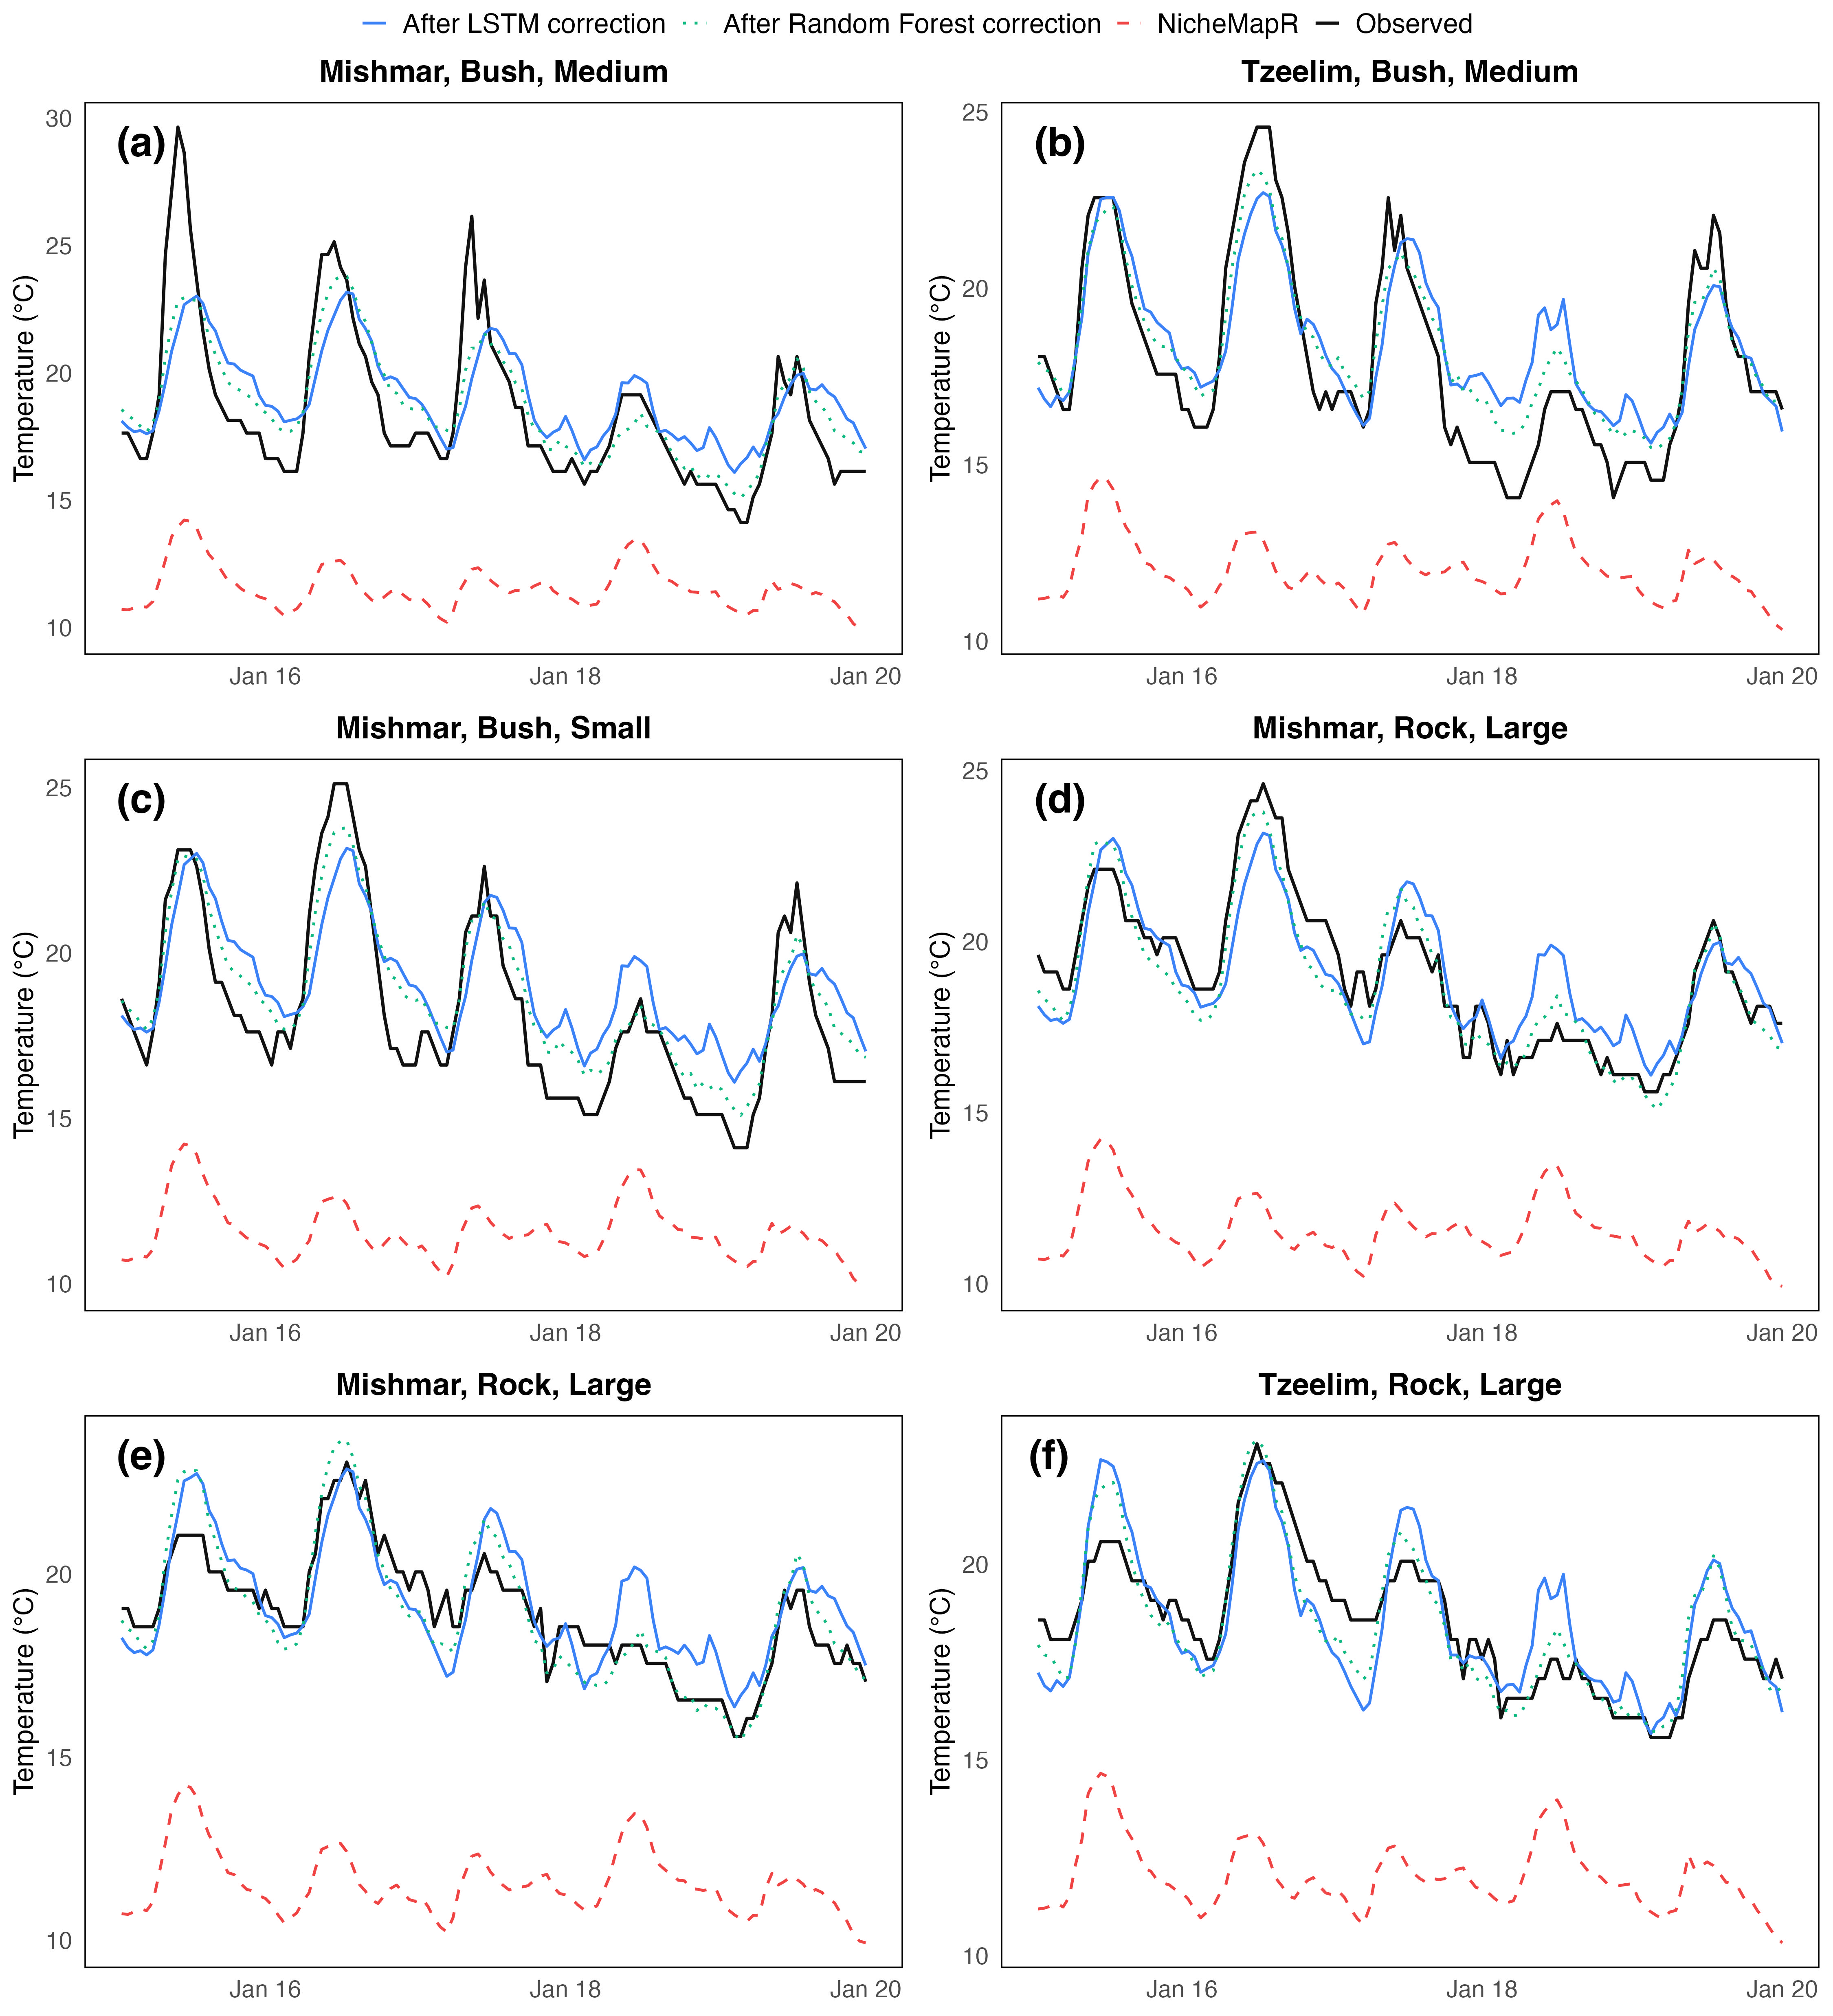
\includegraphics[width=\textwidth,height=0.85\textheight,keepaspectratio]{scenario_6_desert_pooled/prediction_examples_desert_pooled.jpg}
\caption{\textbf{Prediction Examples Desert Pooled for Scenario 6.} Time-series prediction examples comparing observed temperatures (black solid line) to the baseline NicheMapR model (red dashed line) and the ML-corrected models (Random Forest in green dotted line, LSTM in blue solid line, if applicable) over a 120-hour window. The pooled RF model (avg ~1.04 °C, ~87.6\% improvement) substantially outperforms the single-logger baseline from Scenario 3 (1.884 °C, 73.9\%), but uses vastly more training data (118,753 vs ~450–1,570 rows), making the comparison volume-confounded. Performance is virtually identical to the specialized per-region models in Scenario 7 (~1.05 °C avg RF), confirming that pooling all 48 desert loggers into one model does not hurt accuracy relative to region-specific models.}
\end{figure}

\clearpage
\begin{figure}[H]
\centering
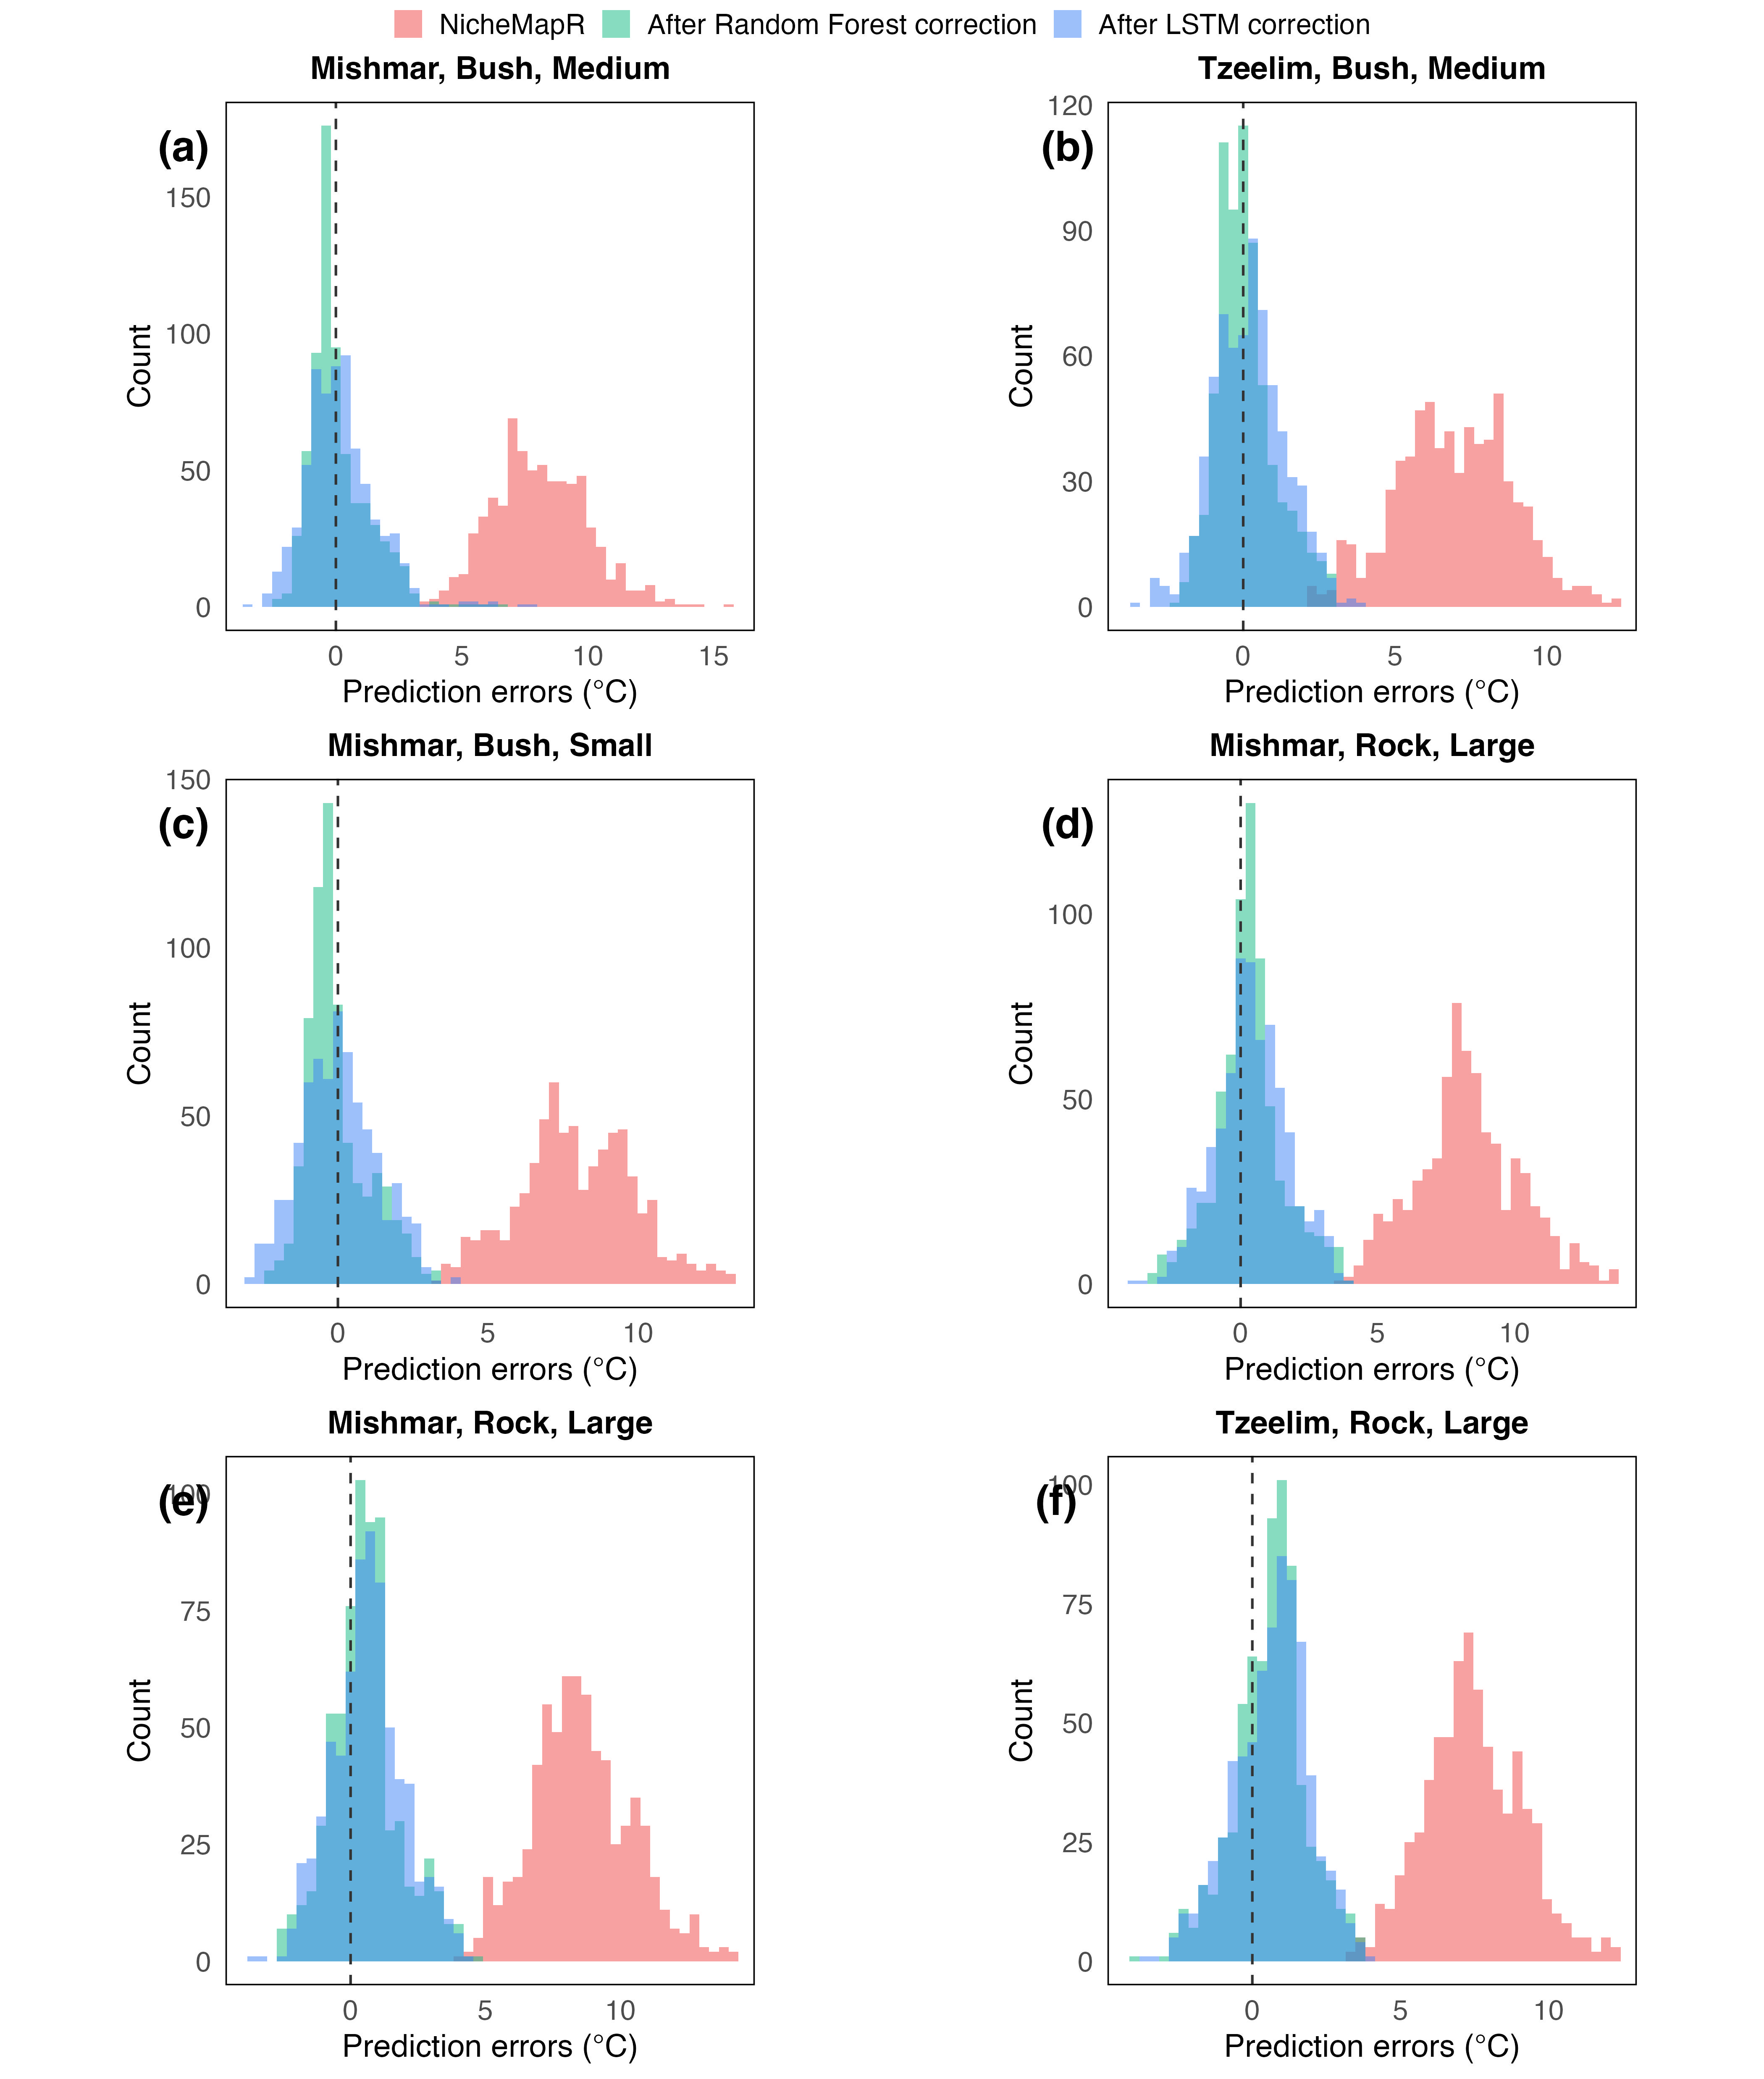
\includegraphics[width=\textwidth,height=0.85\textheight,keepaspectratio]{scenario_6_desert_pooled/residual_histogram_desert_pooled.jpg}
\caption{\textbf{Residual Histogram Desert Pooled for Scenario 6.} Distribution of prediction errors (residuals) comparing the baseline NicheMapR model (red) to the ML-corrected models (Random Forest in green, LSTM in blue, if applicable). A narrower distribution centered at zero indicates better performance. The pooled RF model (avg ~1.04 °C, ~87.6\% improvement) substantially outperforms the single-logger baseline from Scenario 3 (1.884 °C, 73.9\%), but uses vastly more training data (118,753 vs ~450–1,570 rows), making the comparison volume-confounded. Performance is virtually identical to the specialized per-region models in Scenario 7 (~1.05 °C avg RF), confirming that pooling all 48 desert loggers into one model does not hurt accuracy relative to region-specific models.}
\end{figure}

\clearpage

\section{Scenario 7: Judean Desert — Specialized (Location-Specific) Models}

\textbf{Description:} Location-specific models are trained on each of the two desert regions (Mishmar, Tzeelim) and tested on local sensor sites, aggregated by microhabitat type.

**Comparison baselines:**
- Scenario 3 (single loggers): RF RMSE = 1.884 °C, 73.9\% improvement, ~448–1,570 train rows per logger.
- Scenario 6 (pooled, all 48 loggers): RF avg ~1.04 °C, ~87.6\% improvement, 118,753 train rows.

\clearpage
\begin{figure}[H]
\centering
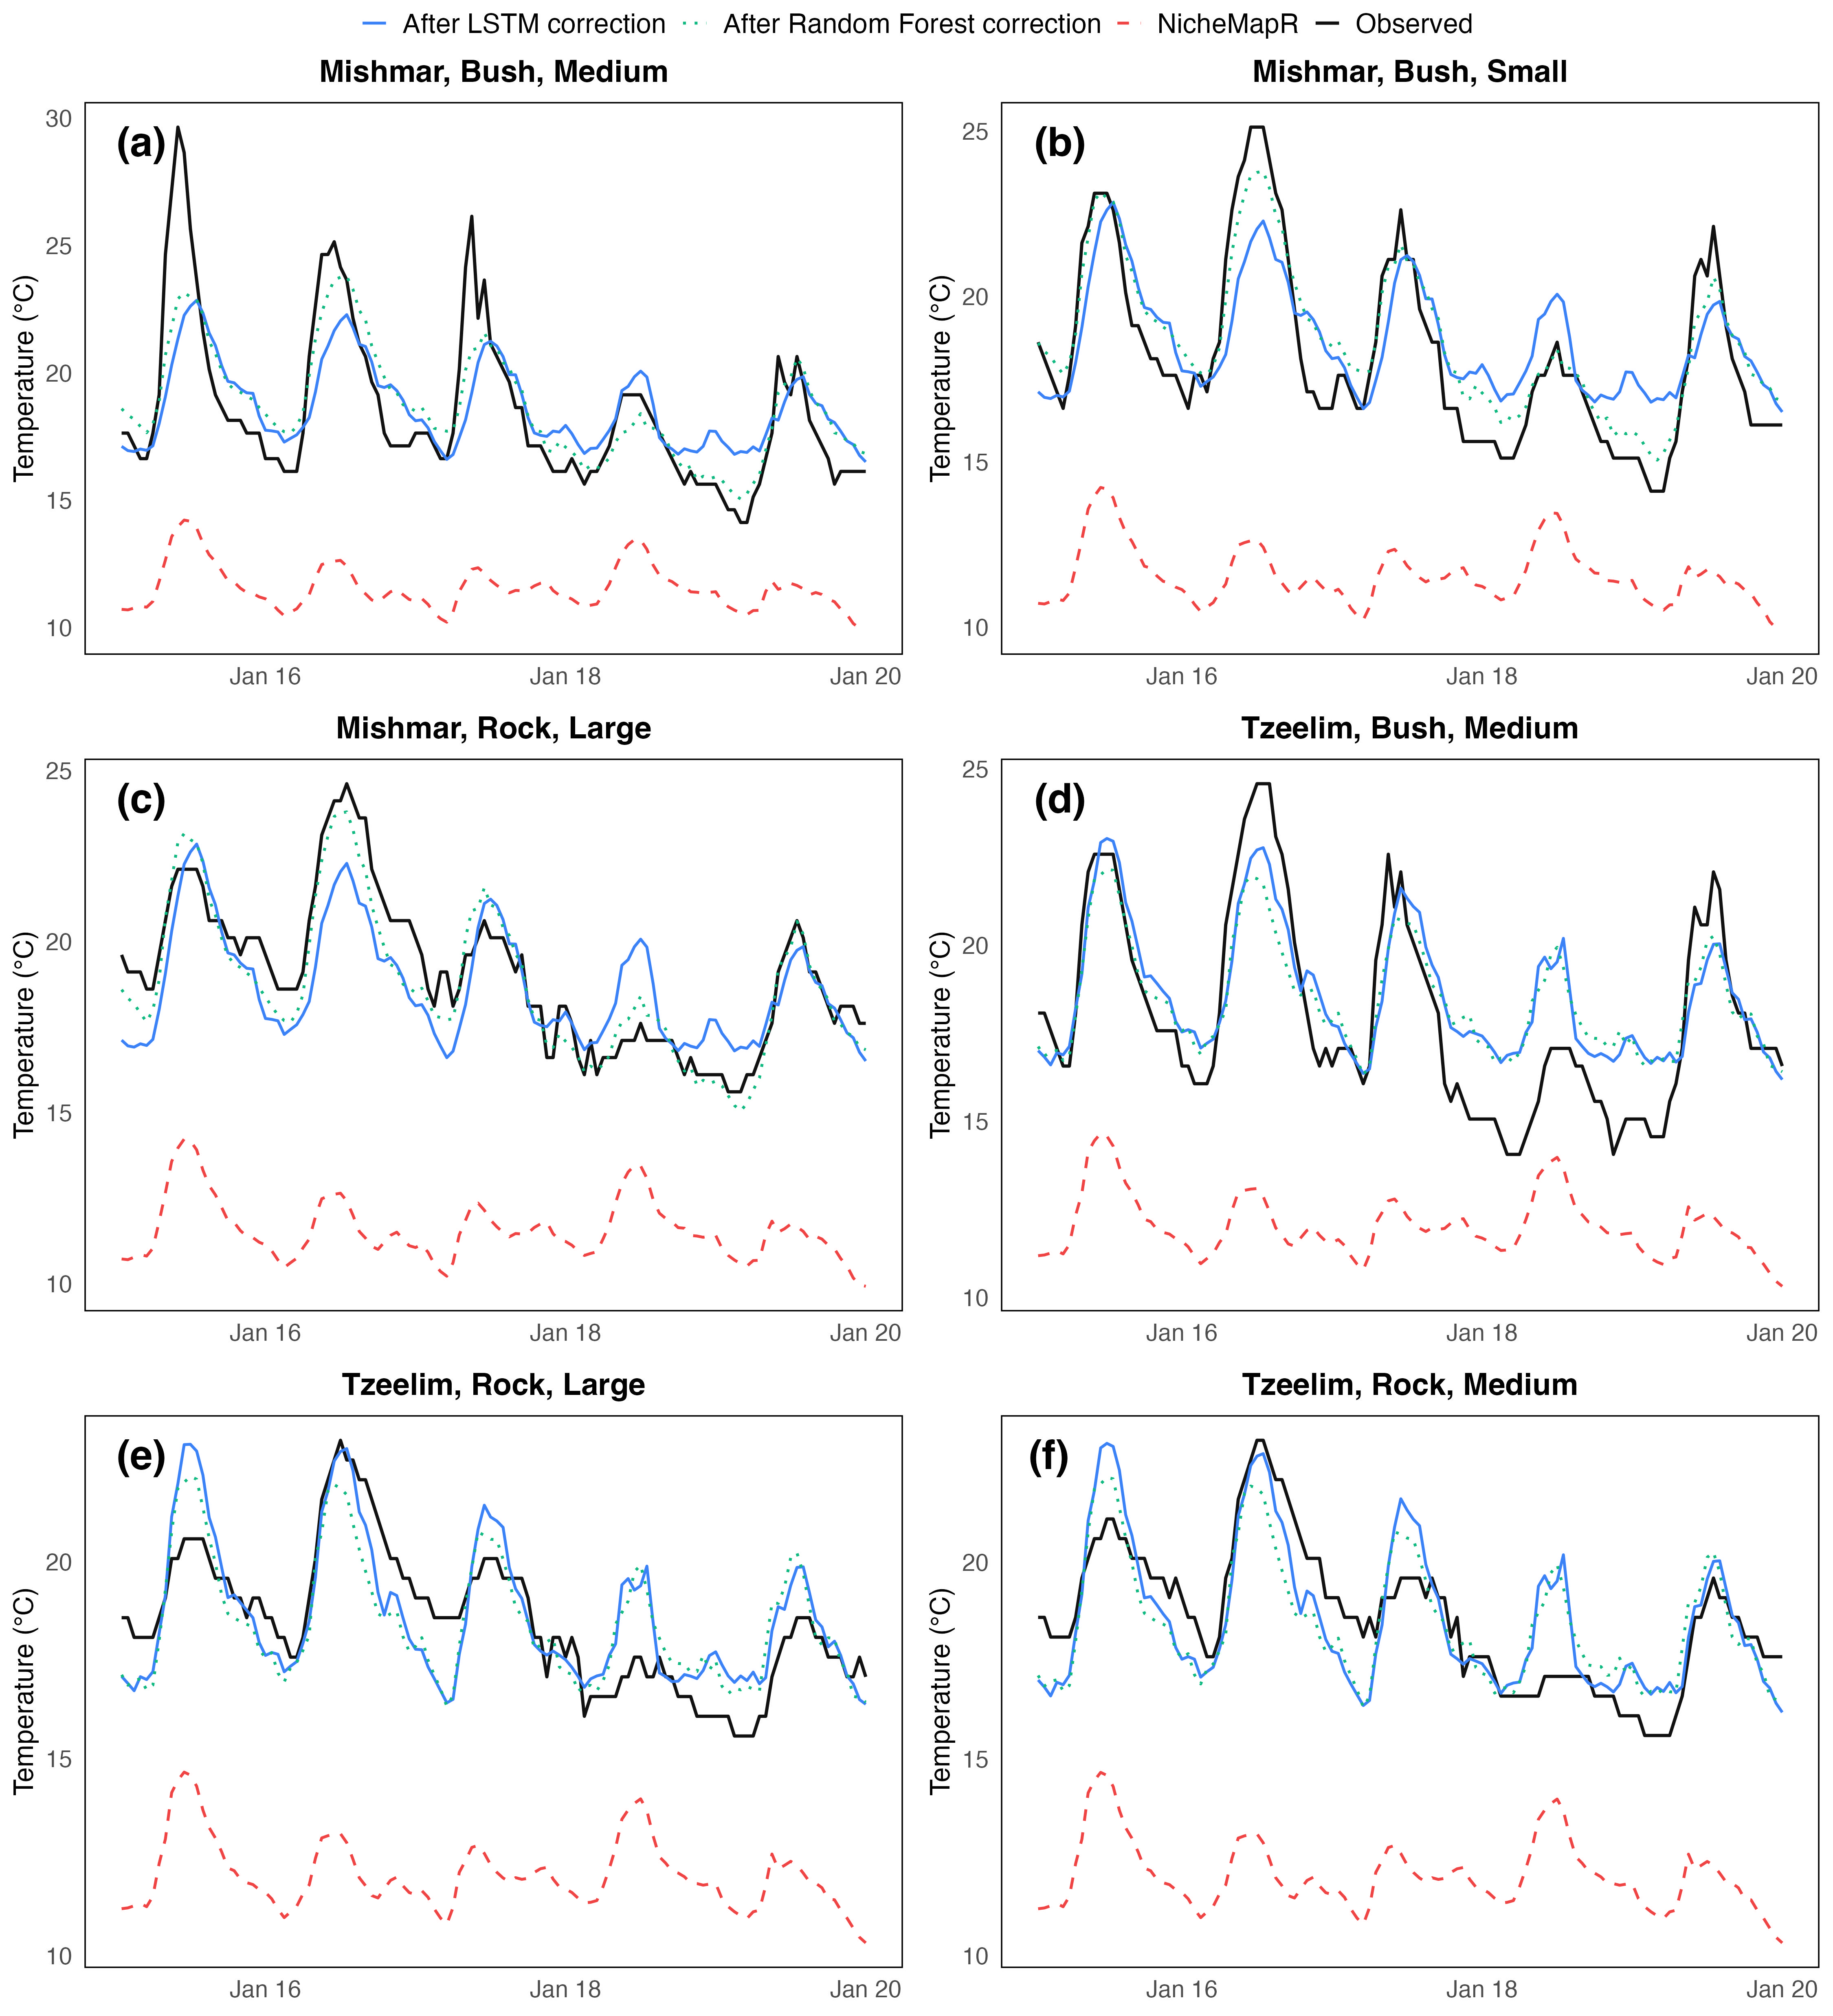
\includegraphics[width=\textwidth,height=0.85\textheight,keepaspectratio]{scenario_7_desert_specialized/prediction_examples_desert_specialized.jpg}
\caption{\textbf{Prediction Examples Desert Specialized for Scenario 7.} Time-series prediction examples comparing observed temperatures (black solid line) to the baseline NicheMapR model (red dashed line) and the ML-corrected models (Random Forest in green dotted line, LSTM in blue solid line, if applicable) over a 120-hour window. Specialized RF models (avg ~1.05 °C, ~87.5\% improvement) substantially outperform the single-logger baseline from Scenario 3 (1.884 °C, 73.9\%), but use 56,668–81,428 rows vs ~450–1,570 per single logger, making the comparison volume-confounded. Performance is virtually identical to the pooled model in Scenario 6 (~1.04 °C avg), confirming that region-specific specialisation adds no measurable benefit over the fully pooled model for Random Forest correction in the Judean Desert.}
\end{figure}

\clearpage
\begin{figure}[H]
\centering
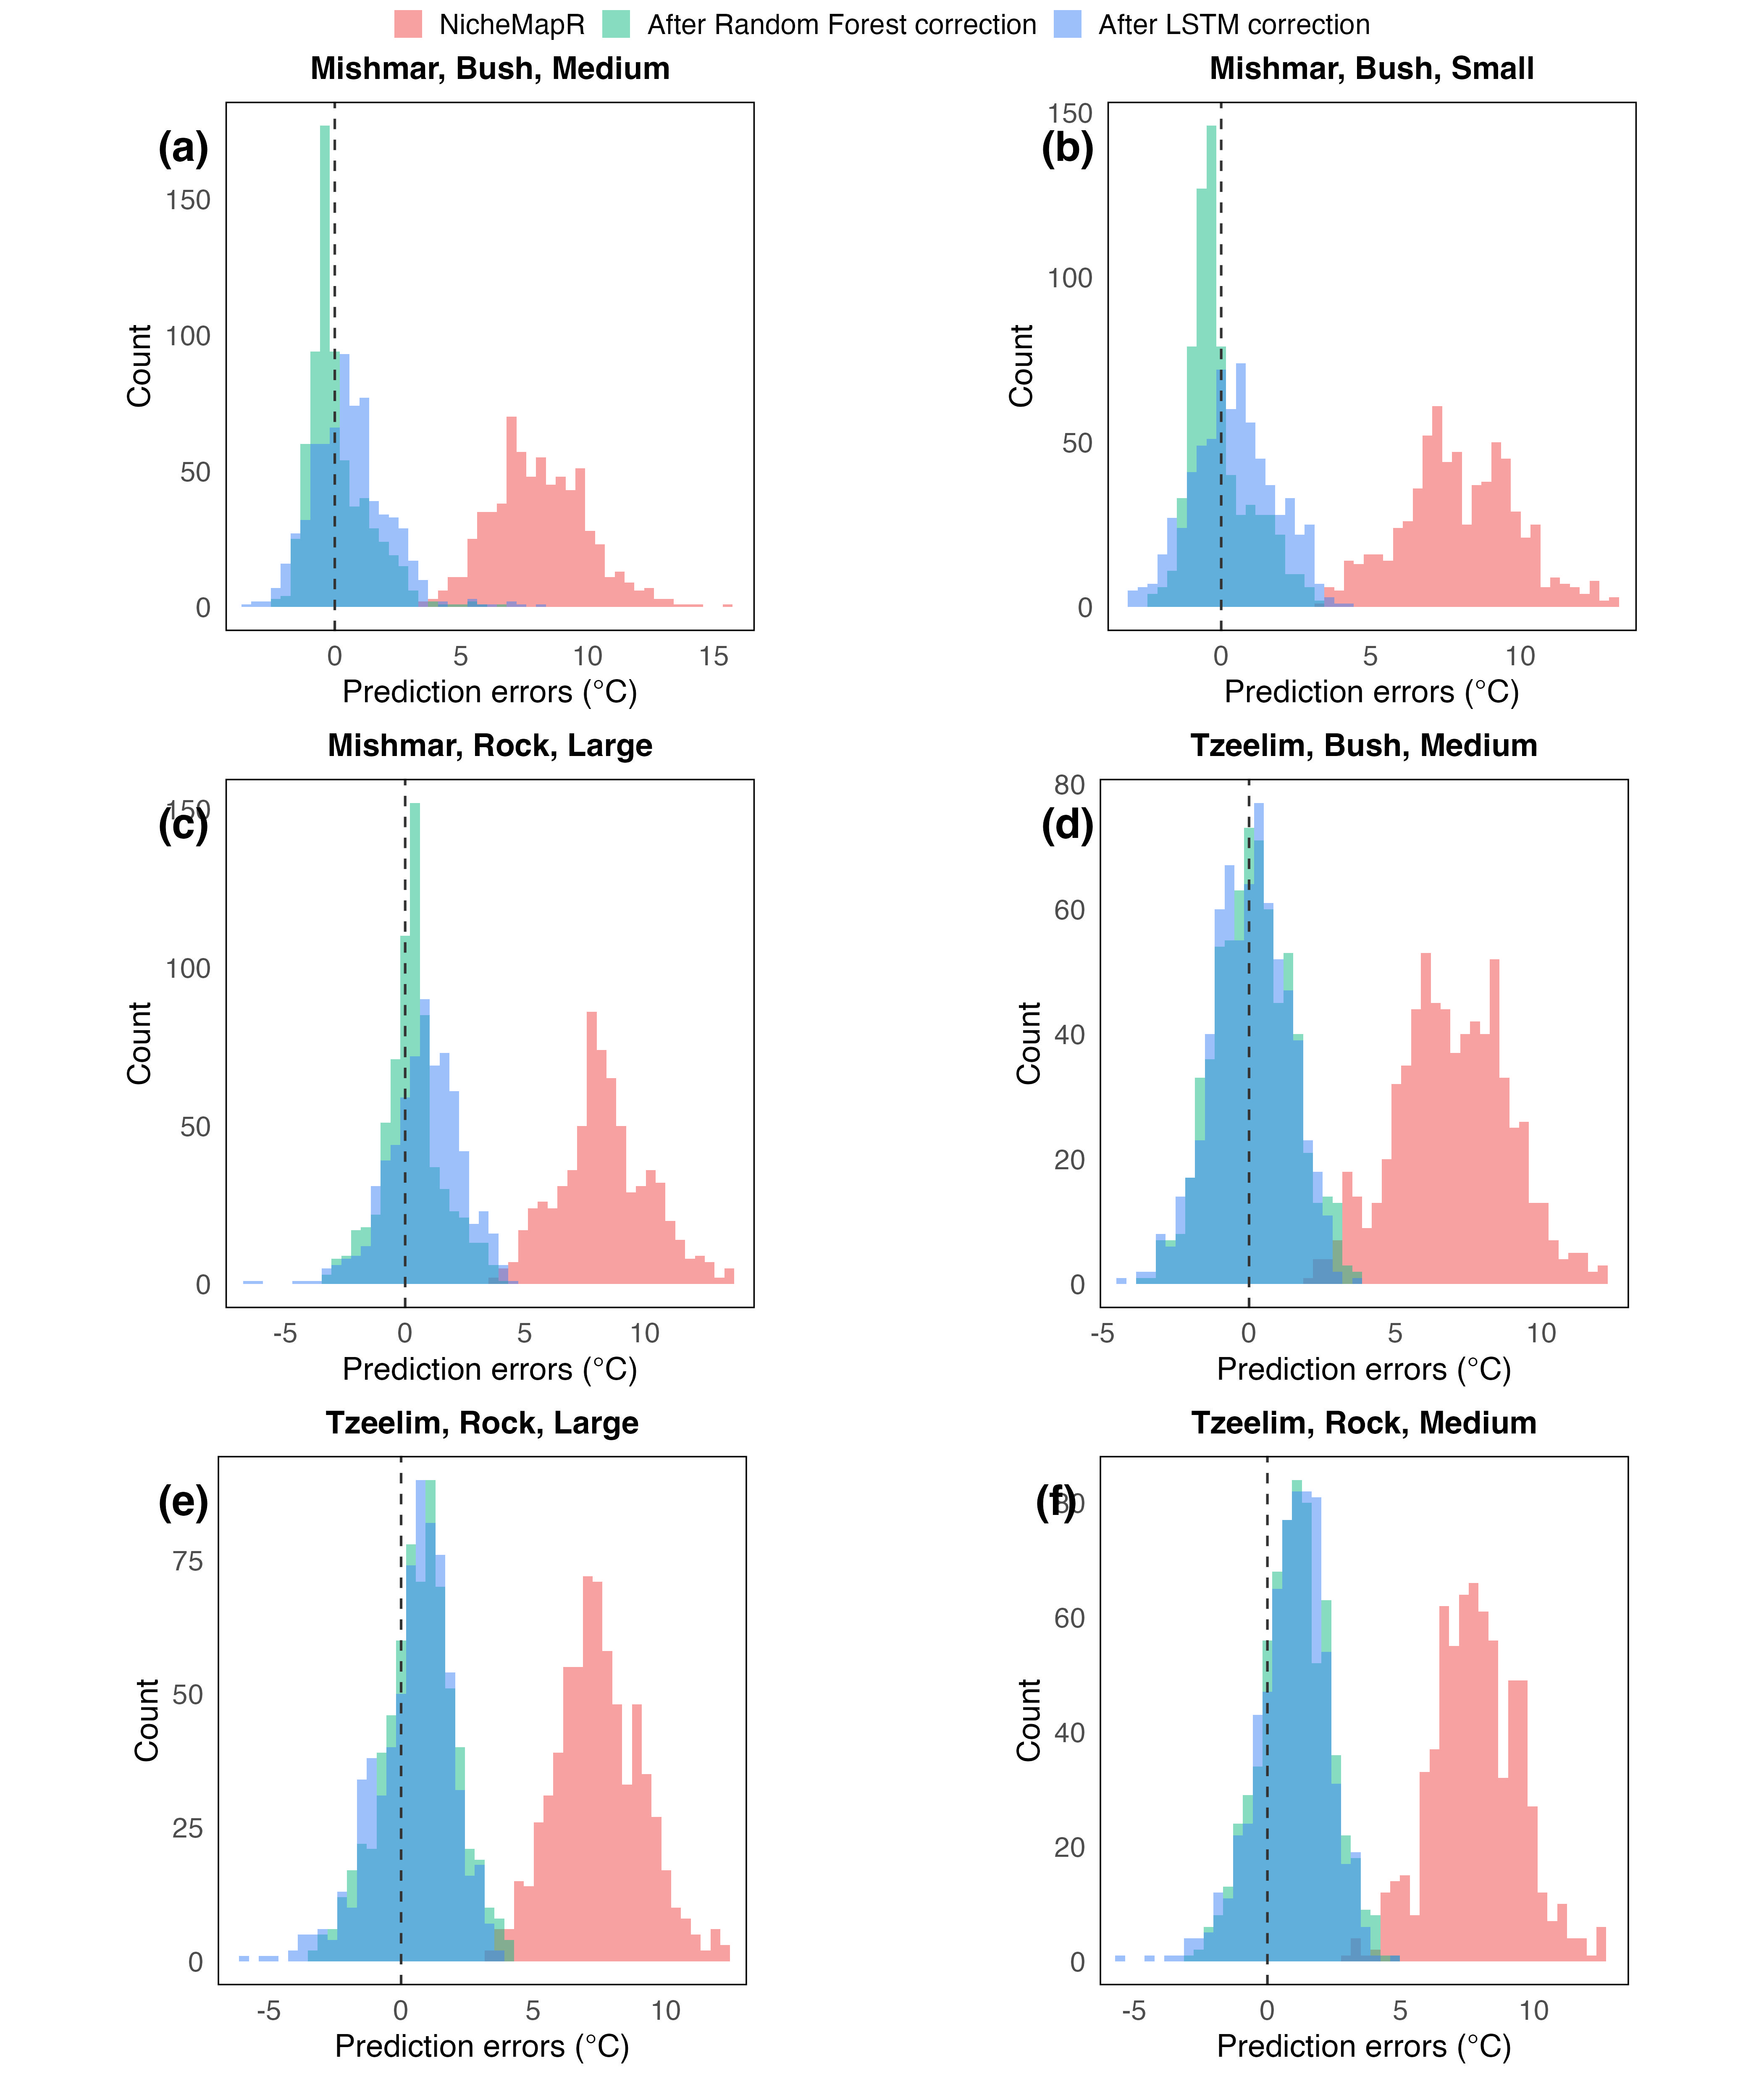
\includegraphics[width=\textwidth,height=0.85\textheight,keepaspectratio]{scenario_7_desert_specialized/residual_histogram_desert_specialized.jpg}
\caption{\textbf{Residual Histogram Desert Specialized for Scenario 7.} Distribution of prediction errors (residuals) comparing the baseline NicheMapR model (red) to the ML-corrected models (Random Forest in green, LSTM in blue, if applicable). A narrower distribution centered at zero indicates better performance. Specialized RF models (avg ~1.05 °C, ~87.5\% improvement) substantially outperform the single-logger baseline from Scenario 3 (1.884 °C, 73.9\%), but use 56,668–81,428 rows vs ~450–1,570 per single logger, making the comparison volume-confounded. Performance is virtually identical to the pooled model in Scenario 6 (~1.04 °C avg), confirming that region-specific specialisation adds no measurable benefit over the fully pooled model for Random Forest correction in the Judean Desert.}
\end{figure}

\clearpage

\section{Scenario 8: Zero-Shot Spatial Transfer — Training on Nearby Sites}

\textbf{Description:} \#\# Motivation
In practice, users often want to correct NicheMapR predictions at a **new location where no temperature logger has been deployed**. This scenario evaluates whether a Random Forest model trained on data from neighboring sites can provide meaningful correction at an unseen target site.

**Comparison baseline — Scenario 2 (single logger, Ashkelon 15 m only):** RF RMSE = 3.06 °C,
62.6\% improvement, ~1,405 train rows. The "Specialized (Local Data)" condition below uses
all Ashkelon loggers combined (~4,631 rows), so it already has ~3× more data than the
Scenario 2 single-logger baseline.

\clearpage
\begin{figure}[H]
\centering
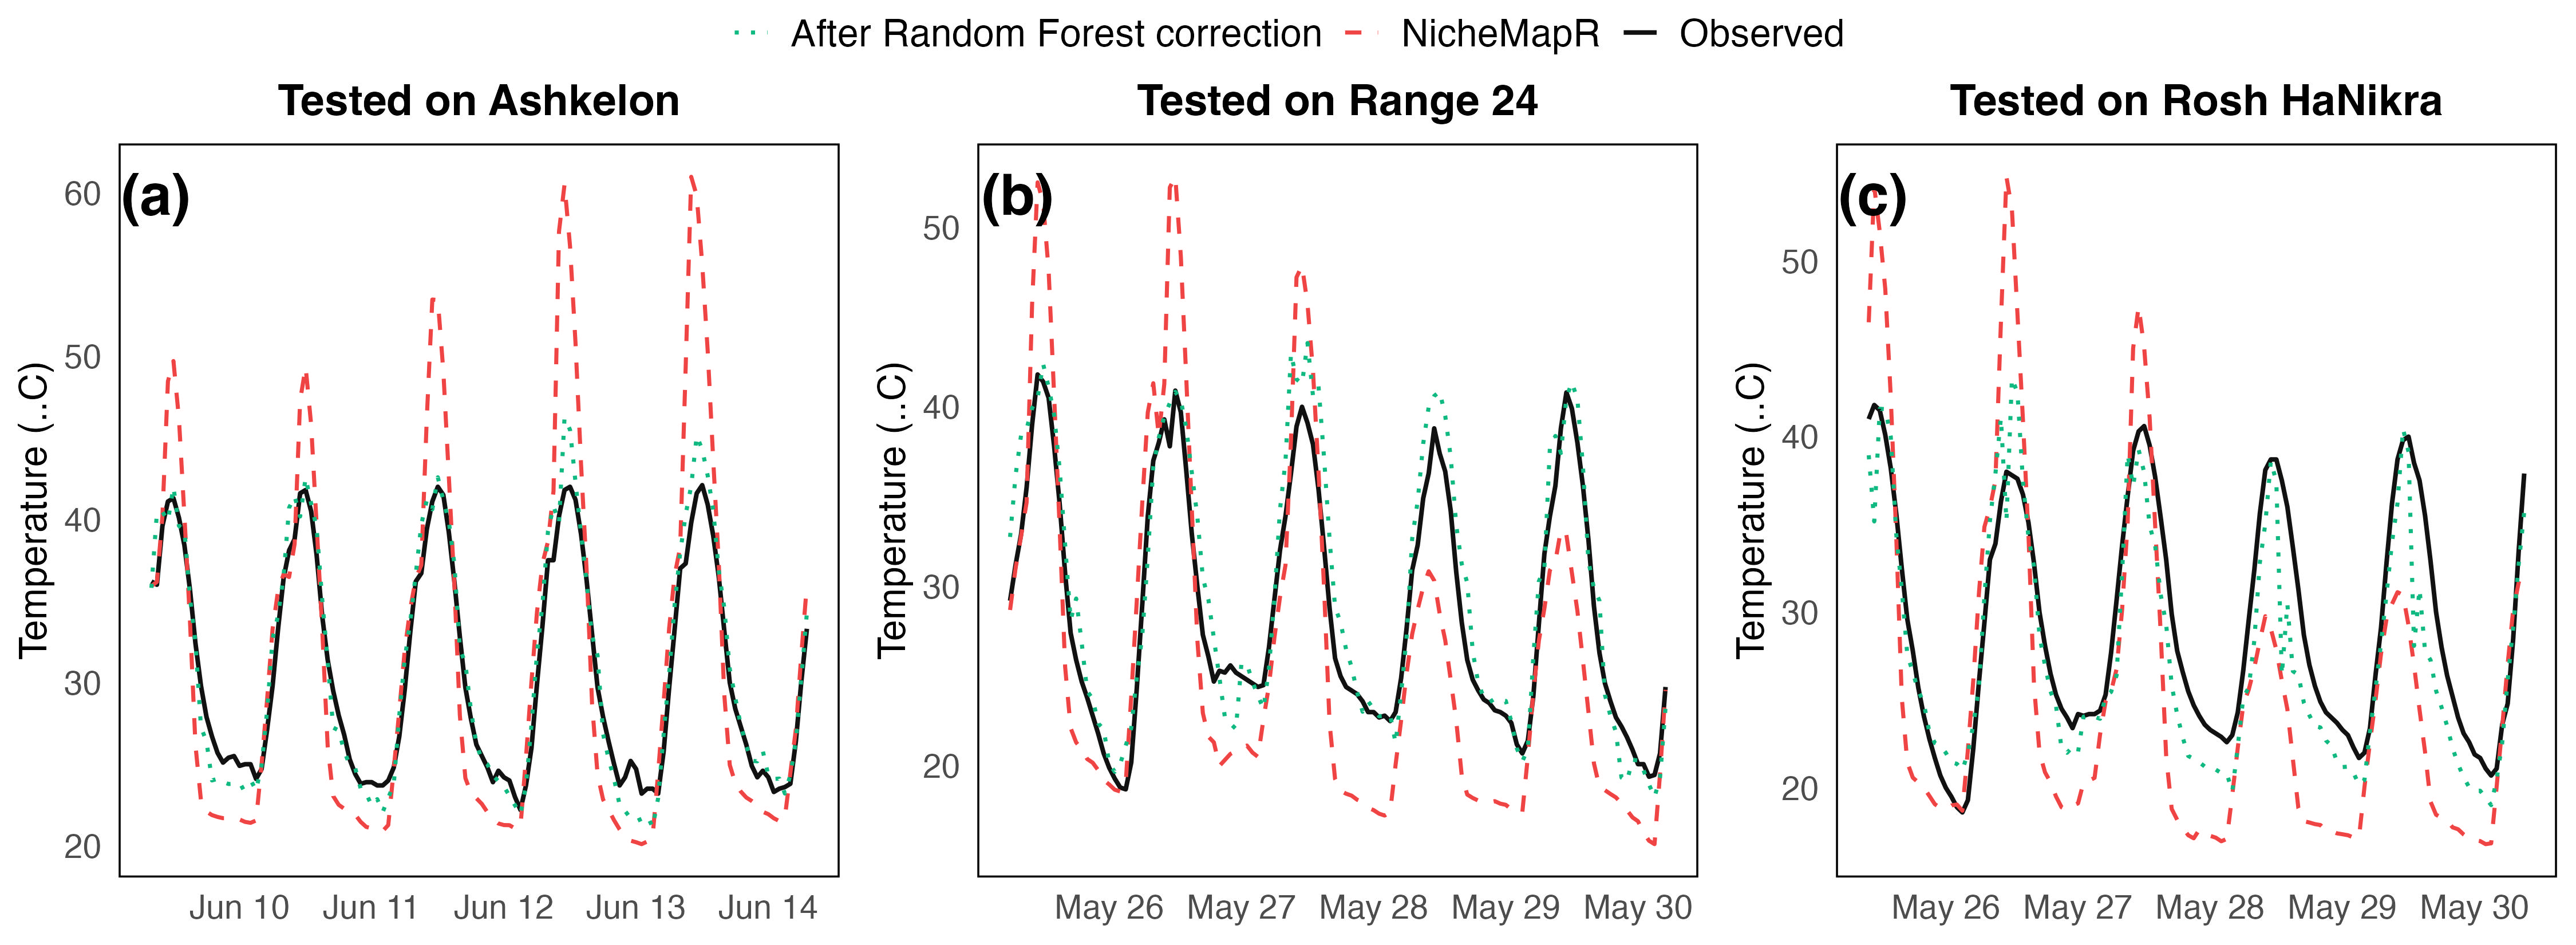
\includegraphics[width=\textwidth,height=0.85\textheight,keepaspectratio]{scenario_8_zero_shot_transfer/prediction_examples_zero_shot.jpg}
\caption{\textbf{Prediction Examples Zero Shot for Scenario 8.} Time-series prediction examples comparing observed temperatures (black solid line) to the baseline NicheMapR model (red dashed line) and the ML-corrected models (Random Forest in green dotted line, LSTM in blue solid line, if applicable) over a 120-hour window. Zero-Shot Transfer Provides Substantial Correction Even without any local training data, the zero-shot model reduces NicheMapR error by 58-68\% across all Beach locations. This confirms that the physical feature representation (radiation, humidity, wind speed, temporal encoding) captures generalizable correction patterns that transfer across sites.}
\end{figure}

\clearpage
\begin{figure}[H]
\centering
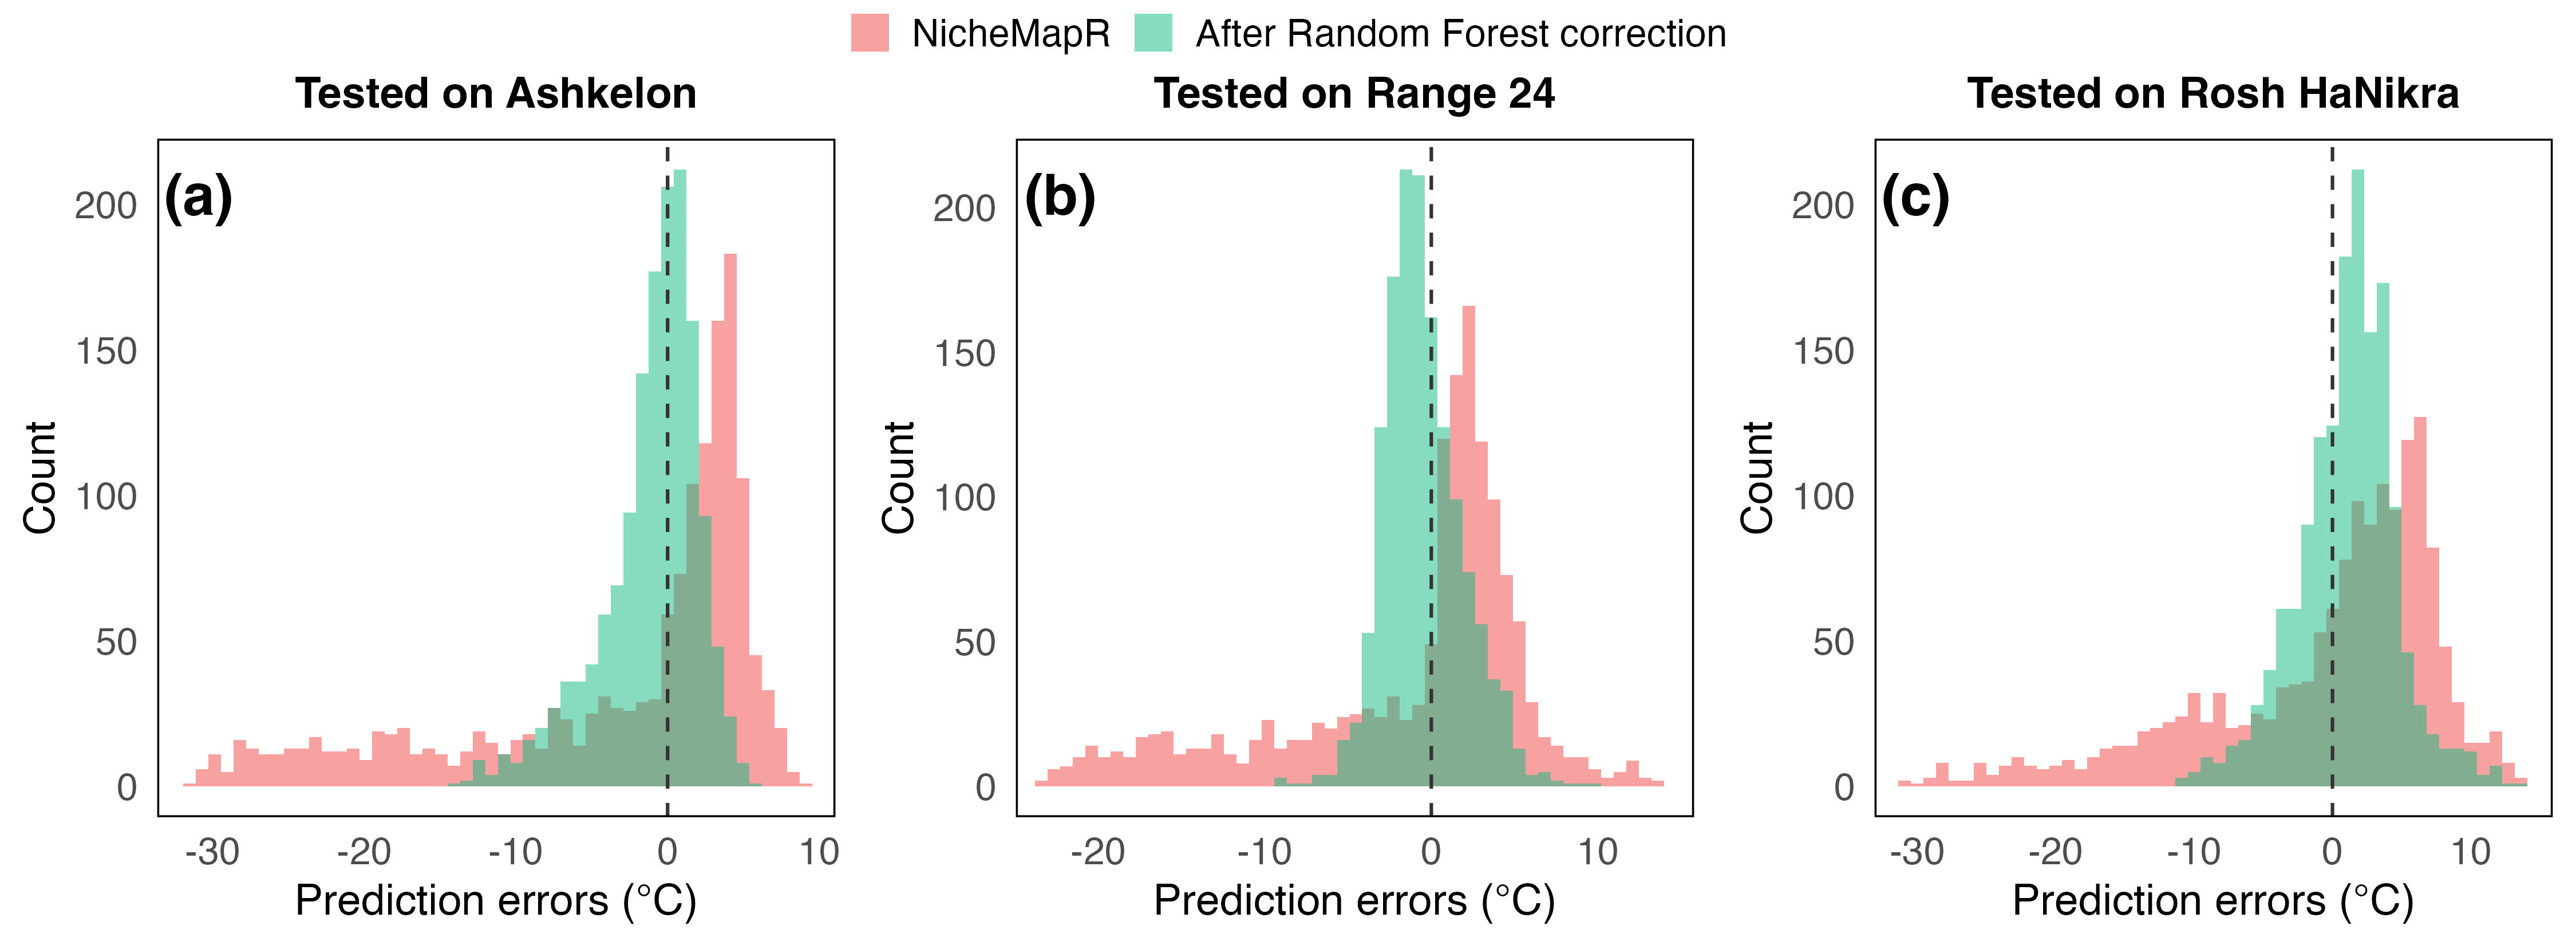
\includegraphics[width=\textwidth,height=0.85\textheight,keepaspectratio]{scenario_8_zero_shot_transfer/residual_histogram_zero_shot.jpg}
\caption{\textbf{Residual Histogram Zero Shot for Scenario 8.} Distribution of prediction errors (residuals) comparing the baseline NicheMapR model (red) to the ML-corrected models (Random Forest in green, LSTM in blue, if applicable). A narrower distribution centered at zero indicates better performance. Zero-Shot Transfer Provides Substantial Correction Even without any local training data, the zero-shot model reduces NicheMapR error by 58-68\% across all Beach locations. This confirms that the physical feature representation (radiation, humidity, wind speed, temporal encoding) captures generalizable correction patterns that transfer across sites.}
\end{figure}

\clearpage

\end{document}
